\documentclass{article}

\usepackage[utf8]{inputenc}
\usepackage[russian]{babel}
\usepackage{graphicx}
\graphicspath{{results/}}
\DeclareGraphicsExtensions{.pdf,.png,.jpg}
\usepackage[unicode, pdftex]{hyperref}
\usepackage{csvsimple}
\usepackage[stable]{footmisc}
\usepackage{subfigure}

\begin{document}

\begin{titlepage}
  \centerline {Санкт-Петербургский политехнический университет}
  \centerline { им. Петра Великого}
  \centerline { }
  \centerline {Институт прикладной математики и механики} 
  \centerline {Кафедра "Прикладная математика"}
  \vfill
  \centerline{\textbf{Отчёт}}
  \centerline{\textbf{по лабораторной работе №4}}
  \centerline{\textbf{по дисциплине}}
  \centerline{\textbf{"Математическая статистика"}}
  \vfill
  \hfill
  \begin{minipage}{0.45\textwidth}
  Выполнил студент:\\
  Дроздова Дарья Александровна\\
  группа: 3630102/80401 \\
  \\
  Проверил:\\
  к.ф.-м.н., доцент \\
  Баженов Александр Николаевич
  \end{minipage}
  \vfill
  \centerline {Санкт-Петербург}   
  \centerline {2021 г.}  
\end{titlepage}

\newpage
\setcounter{page}{2}
\tableofcontents

\newpage
\listoffigures

\newpage
\section{Постановка задачи}
Для 5 распределений:
\begin{itemize}
	\item Нормальное распределение: $N(x,0,1)$
    \item Распределение Коши: $C(x,0,1)$
    \item Распределение Лапласа: $L(x,0,\sqrt{2})$
    \item Распределение Пуассона: $P(k,10)$
    \item Равномерное распределение: $U(x,-\sqrt{3}, \sqrt{3})$
\end{itemize}
Построить выборки мощностью 20, 60 и 100 элементов. Построить для данных выборок эмпирическую функцию распределения и ядерные оценки плотности для непрерывных распределений на отрезке $[-4,4]$, для дискретных на отрезке $[6,14]$

\newpage
\section{Теория}

\subsection{Классификация распределений}
В данной лабораторной работе рассматриваются непрерывные и дискретные распределения. \\
Непрерывные распределения:
\begin{itemize}
    \item Нормальное распределение: $N(x,0,1)$
    \item Распределение Коши: $C(x,0,1)$
    \item Распределение Лапласа: $L(x,0,\sqrt{2})$
    \item Равномерное распределение: $U(x,-\sqrt{3}, \sqrt{3})$
\end{itemize}
Дискретные распределения:
\begin{itemize}
    \item Распределение Пуассона: $P(k,10)$
\end{itemize}

\subsection{Эмпирическая функция распределения}

\subsubsection{Статистический ряд}

Статистический ряд - последовательность различных элементов выборки $z_1, z_2,..., z_k$, расположенных в возрастающем порядке с указанием частот $n_1, n_2,..., n_k$данных элементов. 

\subsection{Эмпирическая (выборочная) функция распределения}

Просуммируем в статистическом ряде, построенном по данной выборке, все частоты $n_i$, для которых элементы $z_i$ меньше $x$, тогда для относительной частоты получаем формулу
$$
P^*(X < x) =\frac{1}{n}\sum_{z_i<x}n_i
$$
следовательно можем получить функцию распределения дискретной случайной величины $X^*$ по следующей формуле
$$
F^*(x) = \frac{1}{n} \sum_{z_i < n} n_i
$$
Эмпирическая функция распределения является оценкой, т. е. приближенным значением, генеральной функции распределения
$$
F_n  ^*(x) \approx F_X(x)
$$

\subsection{Оценка плотности}

Оценка плотности вероятности $f(x)$ - функция $\hat{f}(x)$, построенная на основе выборки, приближенно равная $f(x)$
$$
\hat{f}(x) \approx f(x)
$$

\subsection{Ядерная оценка плотности}

Представим оценку в виде суммы с числом слагаемых, равным объему выборки
$$
\hat{f}_n(x) = \frac{1}{nh_n} \sum_{i=1}^n K \left( \frac{x-x_i}{h_n} \right)
$$
\\
Функция $K(u)$, называемая ядерной, непрерывна и является плотностью вероятности, $x_1,...,x_n$ - элементы выборки, ${h_n}$ - любая последовательность положительных чисел, обладающая свойствами 
$$
\lim_{n \to \infty} k_n = 0; \; \; \lim_{{n \to \infty}}\frac{h_n}{n^{-1}} = \infty
$$
Такие оценки называются непрерывными ядерными
\\
Гауссово (нормальное ядро) определяется по формуле
$$
K(u) = \frac{1}{\sqrt{2\pi}}e^{-\frac{u^2}{2}}
$$
\\
Правило Сильвермана 
$$
h_n = 1.06 \hat{\sigma} n^{\frac{1}{5}}
$$
где $\hat{\sigma}$ - выборочное отклонение

\newpage
\section{Реализация}

Лабораторная работа выполнена на языке программирования Python в среде разработки PyCharm. Для построения выборки используется библиотека skipy, для математических функций - numpy, для построения эмпирической функции распределения - statmodels, для построений графиков - pyplot, seaborn.
\\
\\
Код программы расположен в репозитории GitHub по ссылке: \url{https://github.com/Drozdova-Daria/Math_Stat_Lab4}

\newpage
\section{Результаты}

\subsection{Эмпирическая функция распределения}

\subsubsection{Нормальное распределение}

\begin{figure}[h]
\center{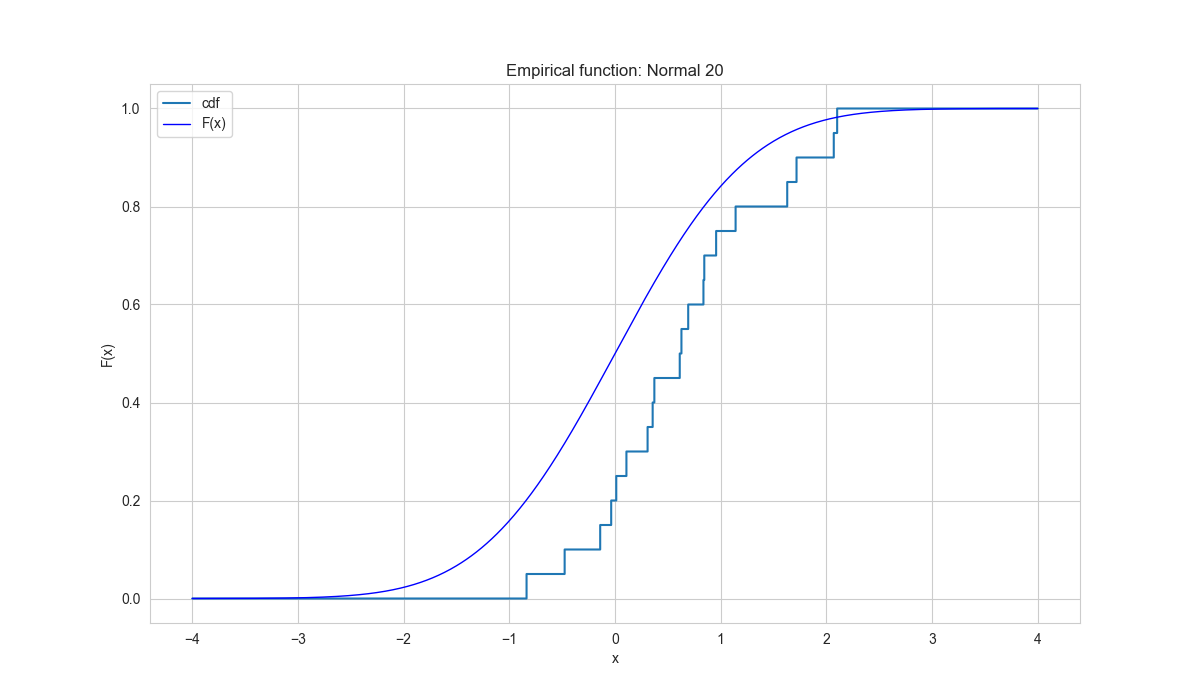
\includegraphics[scale=0.2]{empNormal20}}
\caption{Эмпирическая функция нормального распределения $n=20$}
\end{figure}

\begin{figure}[h]
\center{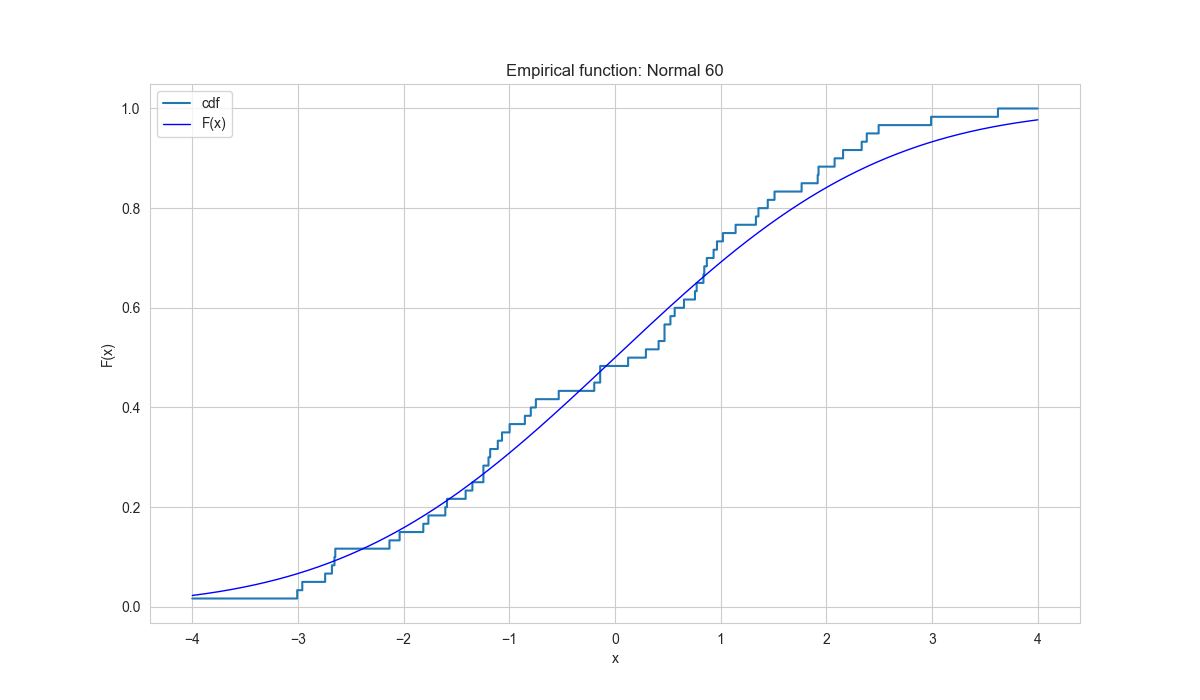
\includegraphics[scale=0.2]{empNormal60}}
\caption{Эмпирическая функция нормального распределения $n=60$}
\end{figure}

\begin{figure}[h]
\center{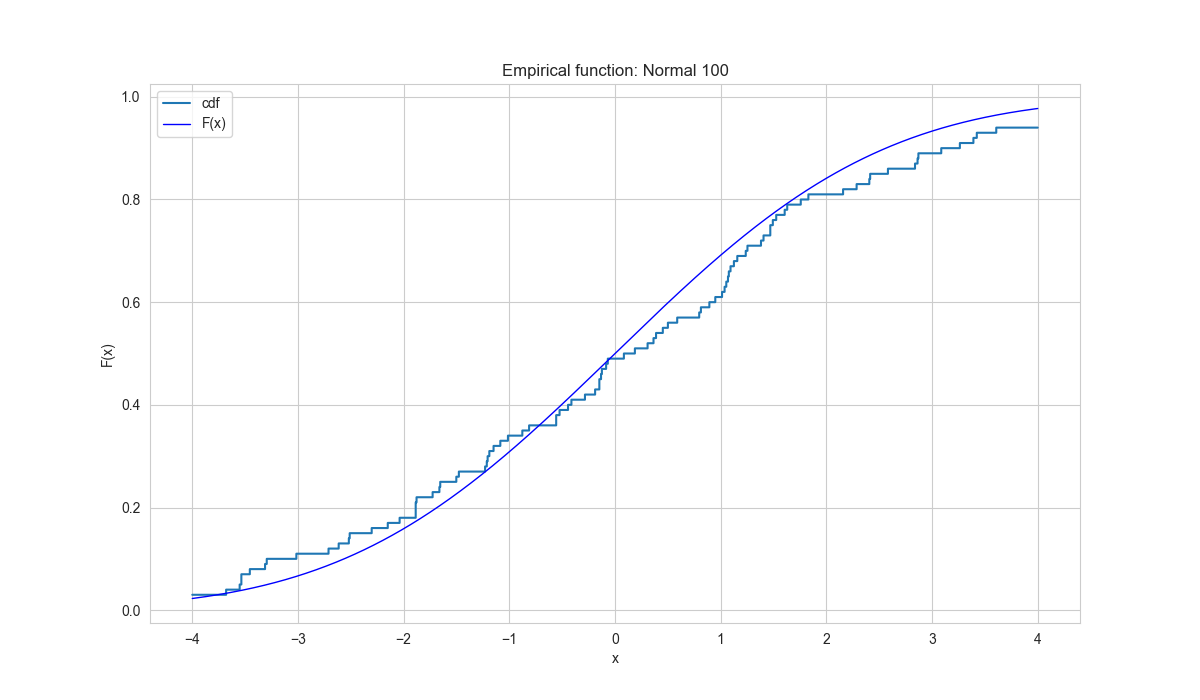
\includegraphics[scale=0.2]{empNormal100}}
\caption{Эмпирическая функция нормального распределения $n=100$}
\end{figure}

\newpage
\subsubsection{Распределение Коши}

\begin{figure}[h]
\center{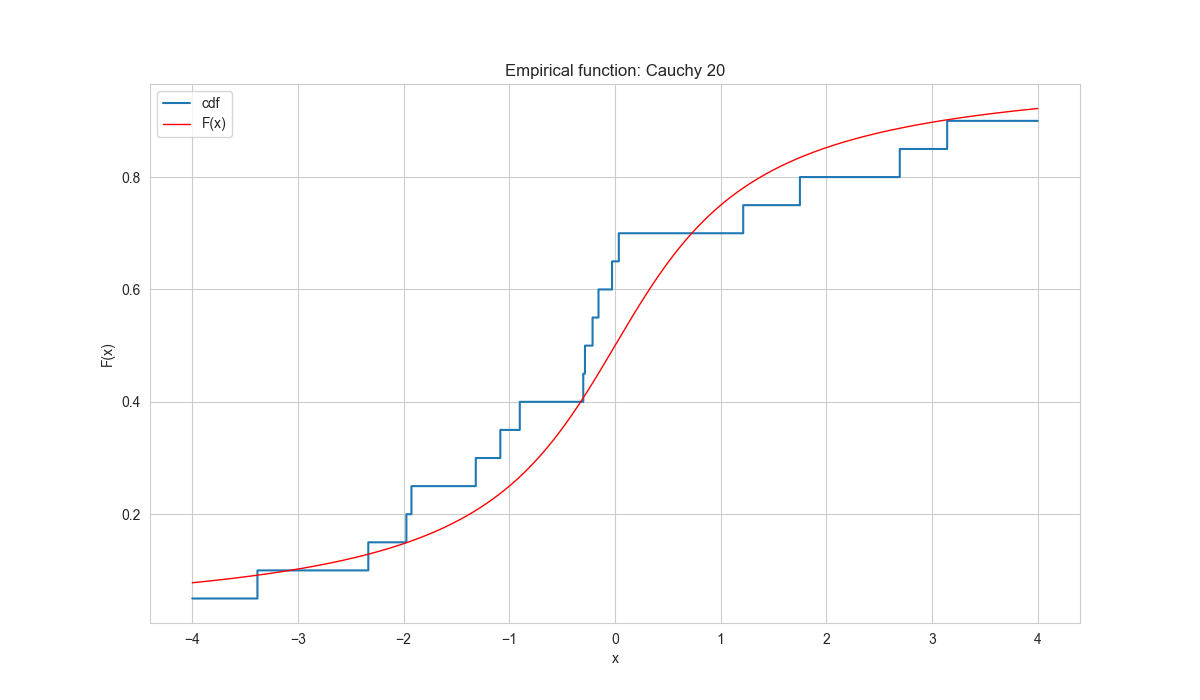
\includegraphics[scale=0.2]{empCauchy20}}
\caption{Эмпирическая функция распределения Коши $n=20$}
\end{figure}

\begin{figure}[h]
\center{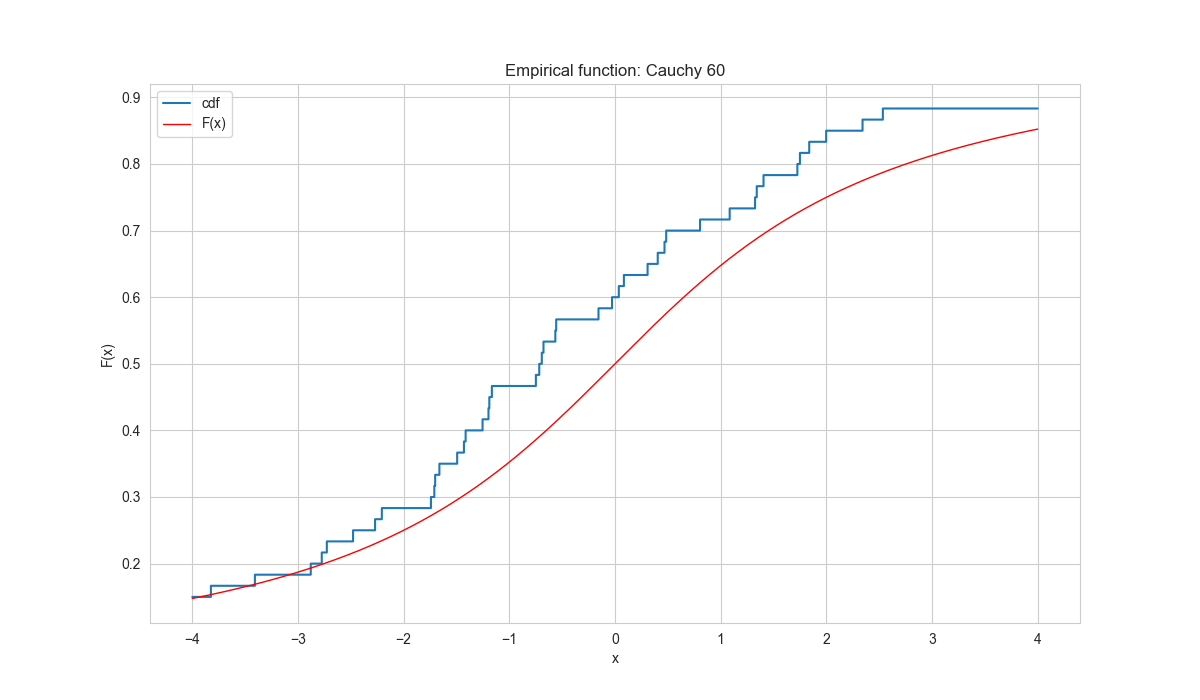
\includegraphics[scale=0.2]{empCauchy60}}
\caption{Эмпирическая функция распределения Коши $n=60$}
\end{figure}

\begin{figure}[h]
\center{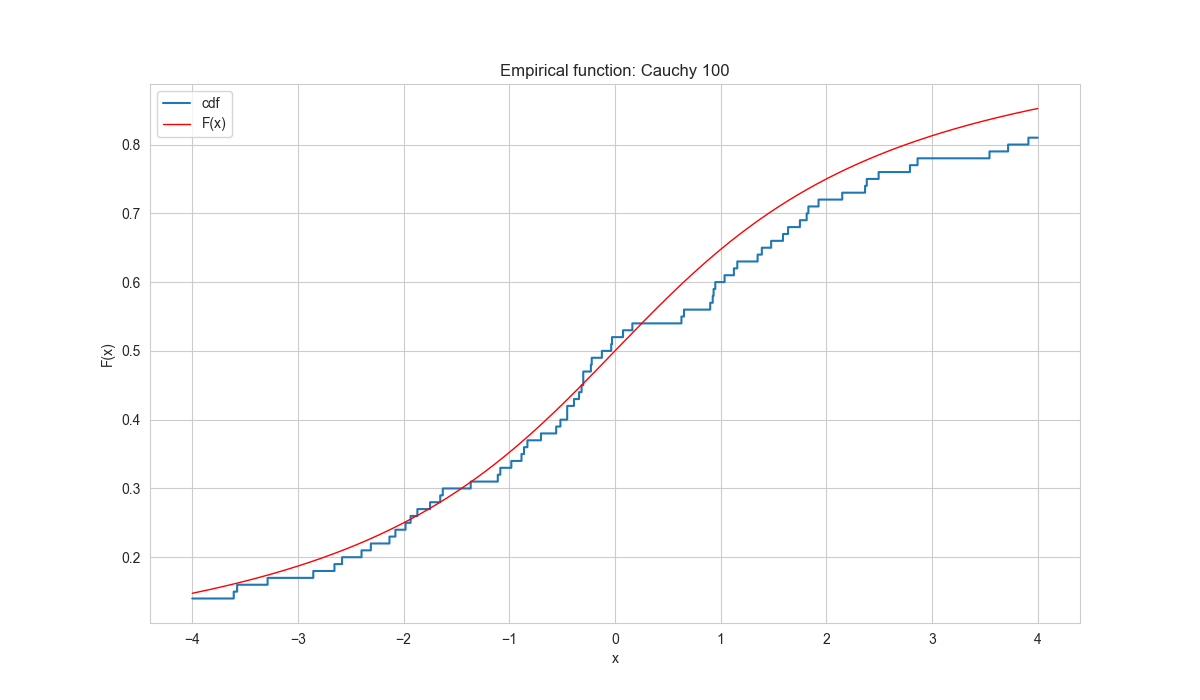
\includegraphics[scale=0.2]{empCauchy100}}
\caption{Эмпирическая функция распределения Коши $n=100$}
\end{figure}

\newpage
\subsubsection{Распределение Лапласа}

\begin{figure}[h]
\center{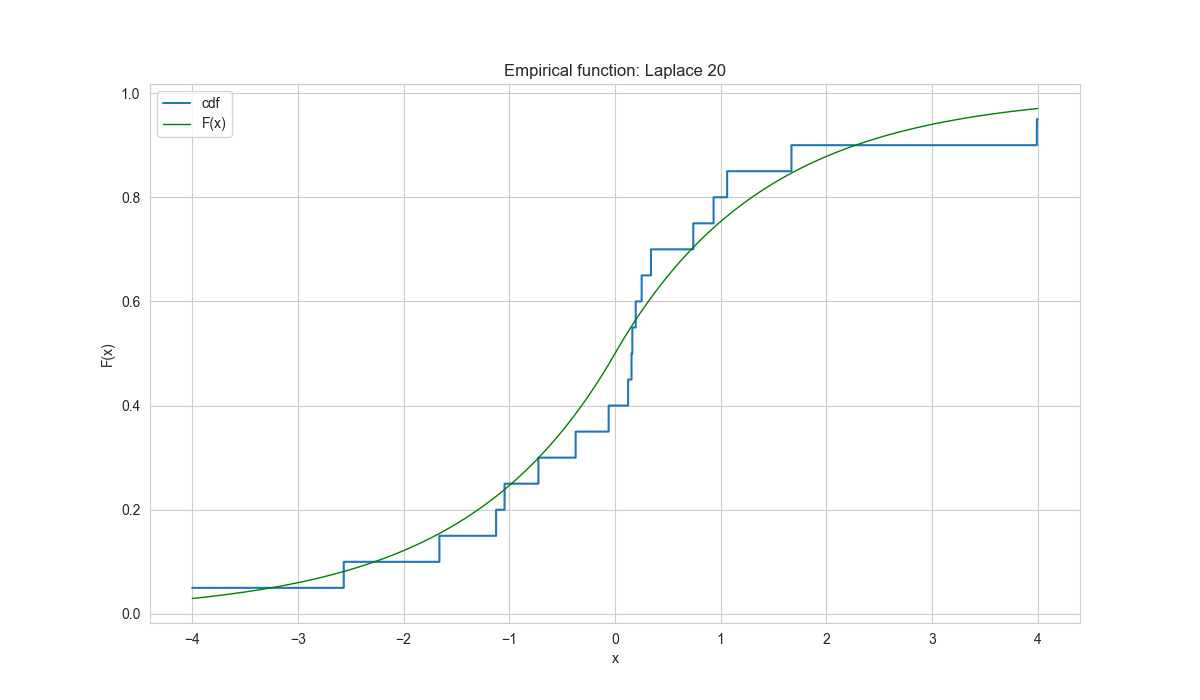
\includegraphics[scale=0.2]{empLaplace20}}
\caption{Эмпирическая функция распределения Лапласа $n=20$}
\end{figure}

\begin{figure}[h]
\center{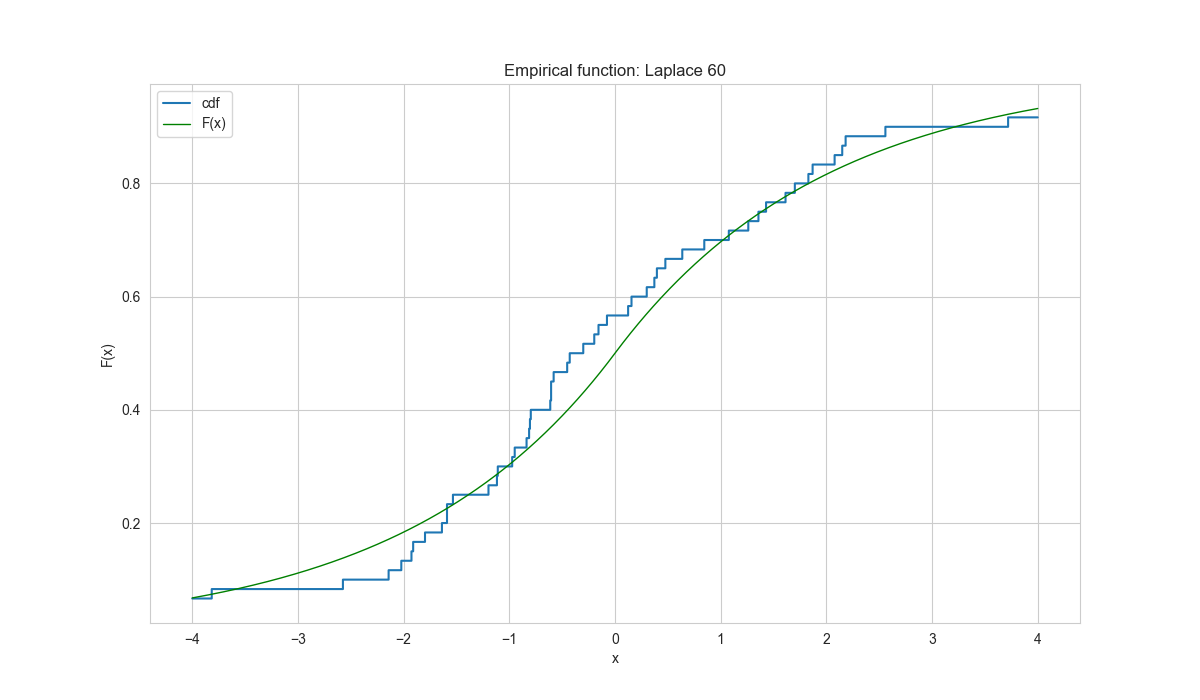
\includegraphics[scale=0.2]{empLaplace60}}
\caption{Эмпирическая функция распределения Лапласа $n=60$}
\end{figure}

\begin{figure}[h]
\center{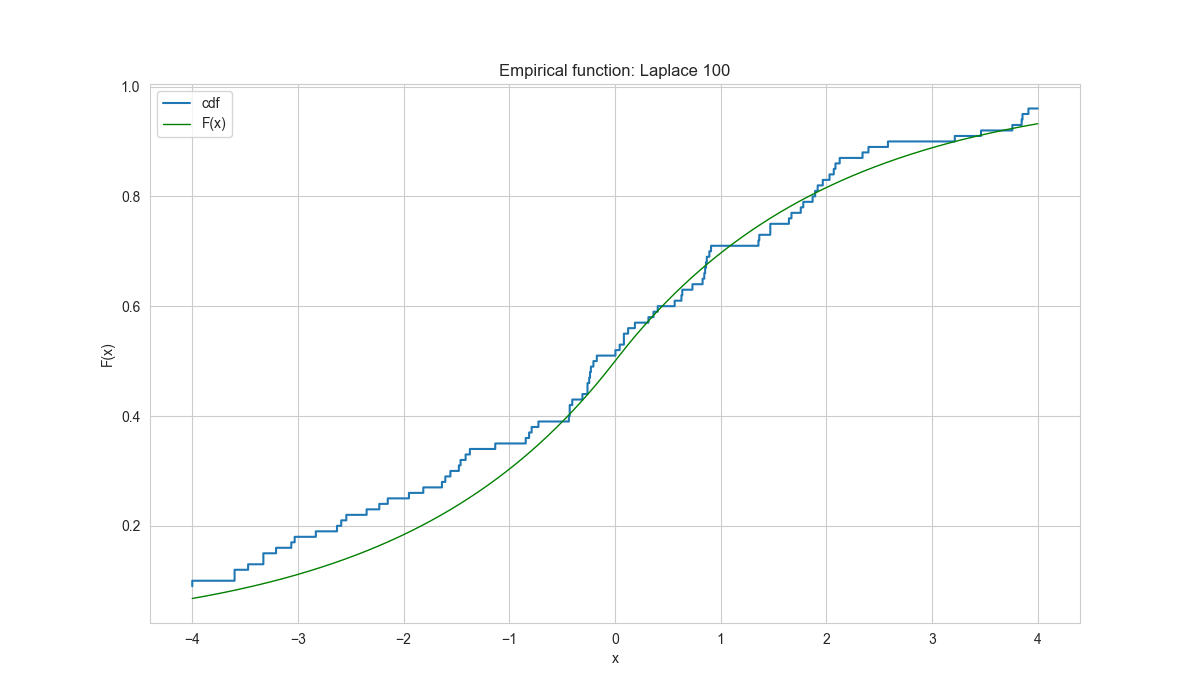
\includegraphics[scale=0.2]{empLaplace100}}
\caption{Эмпирическая функция распределения Лапласа $n=100$}
\end{figure}

\newpage
\subsubsection{Распределение Пуассона}

\begin{figure}[h]
\center{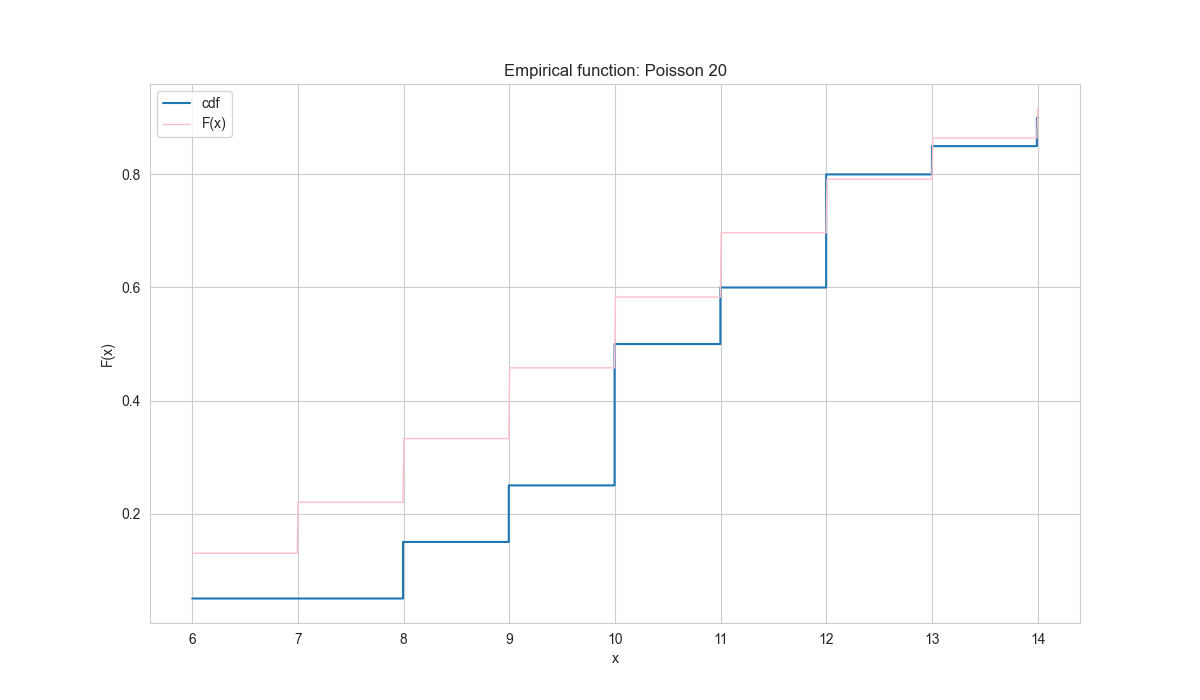
\includegraphics[scale=0.2]{empPoisson20}}
\caption{Эмпирическая функция распределения Пуассона $n=20$}
\end{figure}

\begin{figure}[h]
\center{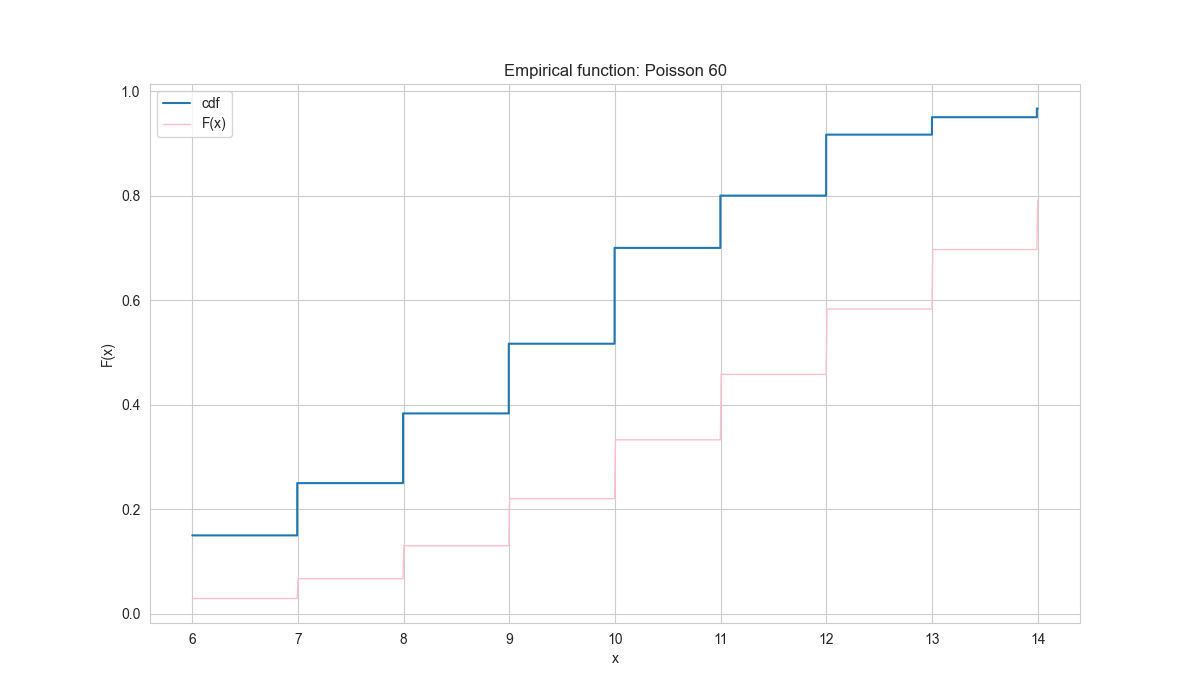
\includegraphics[scale=0.2]{empPoisson60}}
\caption{Эмпирическая функция распределения Пуассона $n=60$}
\end{figure}

\begin{figure}[h]
\center{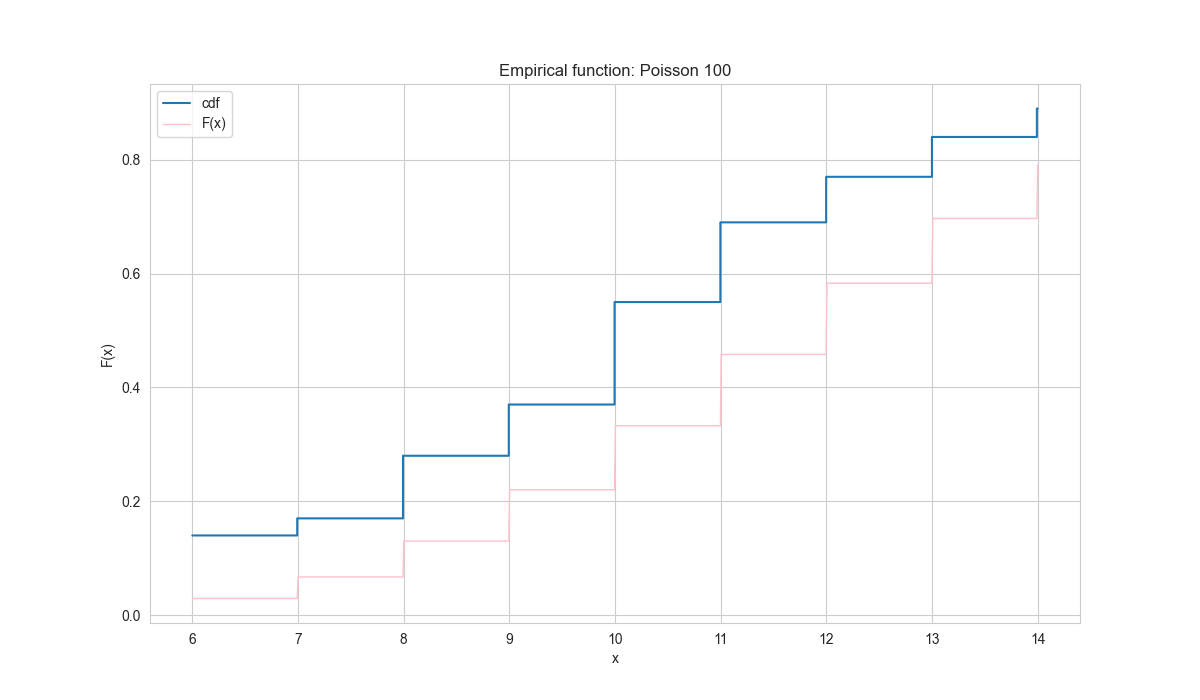
\includegraphics[scale=0.2]{empPoisson100}}
\caption{Эмпирическая функция распределения Пуассона $n=100$}
\end{figure}

\newpage
\subsubsection{Равномерное распределение}

\begin{figure}[h]
\center{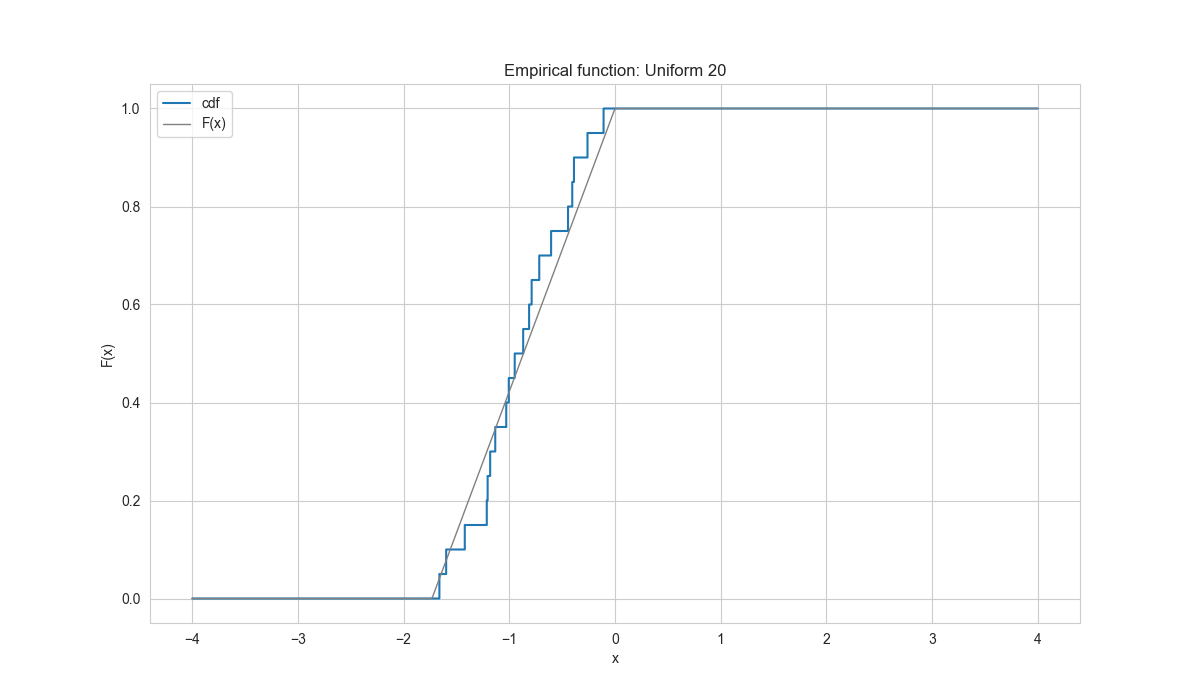
\includegraphics[scale=0.2]{empUniform20}}
\caption{Эмпирическая функция равномерного распределения $n=20$}
\end{figure}

\begin{figure}[h]
\center{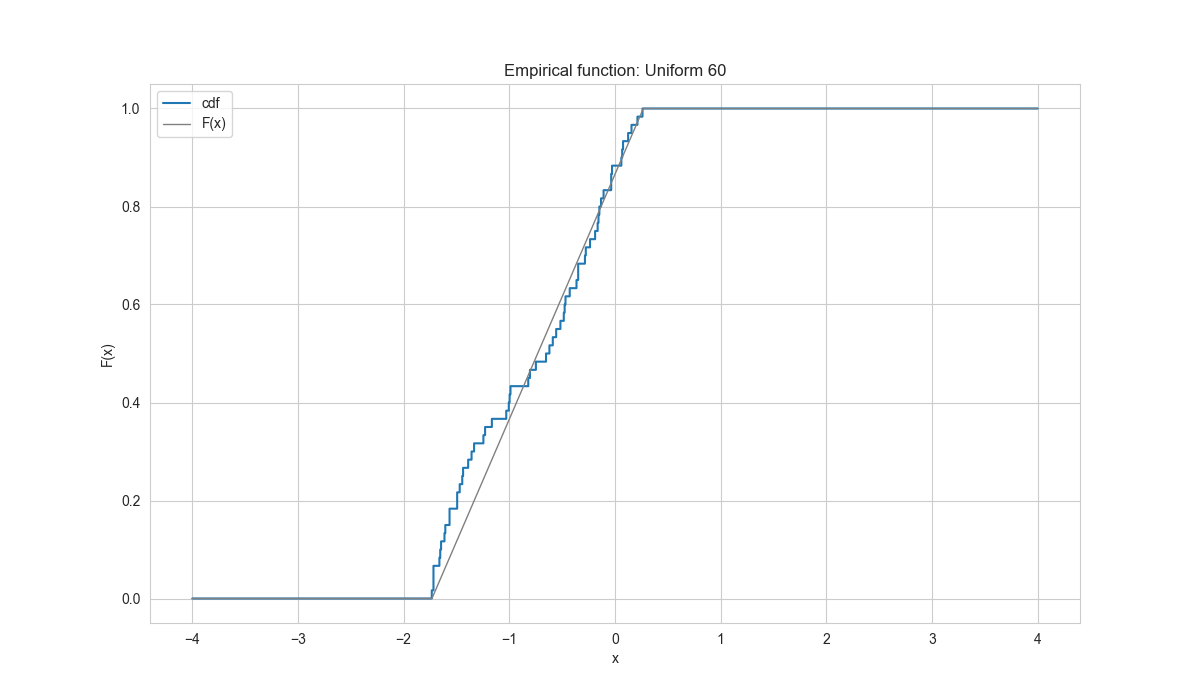
\includegraphics[scale=0.2]{empUniform60}}
\caption{Эмпирическая функция равномерного распределения $n=60$}
\end{figure}

\begin{figure}[h]
\center{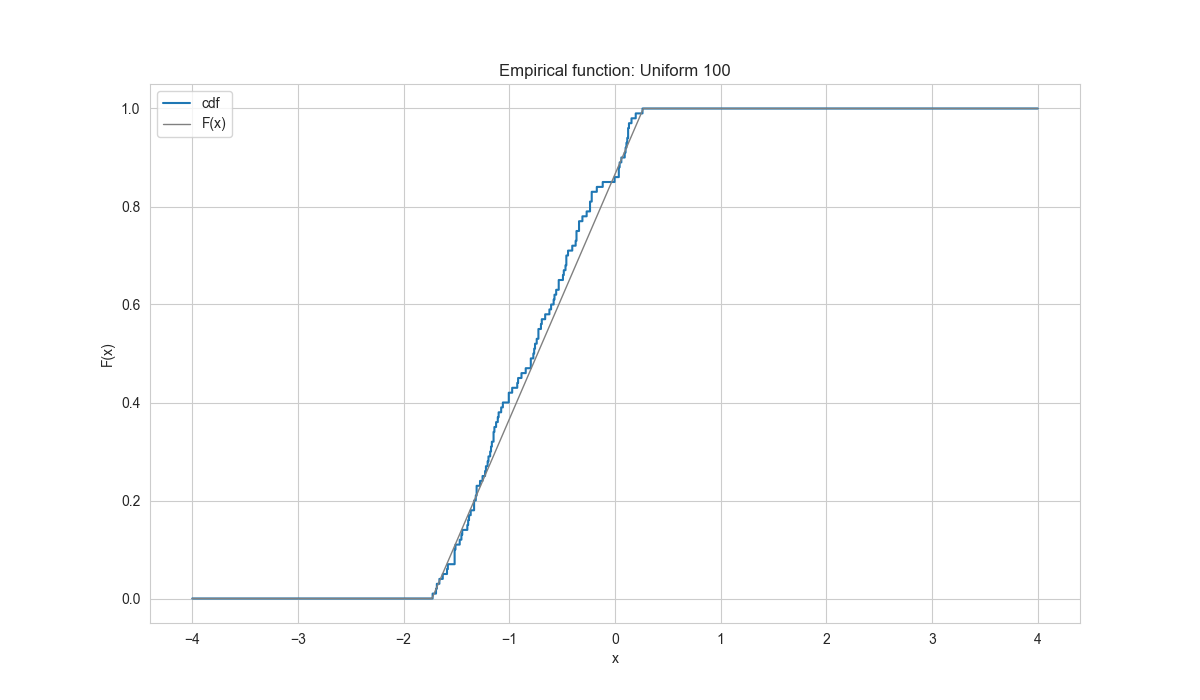
\includegraphics[scale=0.2]{empUniform100}}
\caption{Эмпирическая функция равномерного распределения $n=100$}
\end{figure}

\newpage
\subsection{Ядерная оценка плотности}

\subsubsection{Нормальное распределение}

\begin{figure}[ht!]  
\centering 
\subfigure[]{
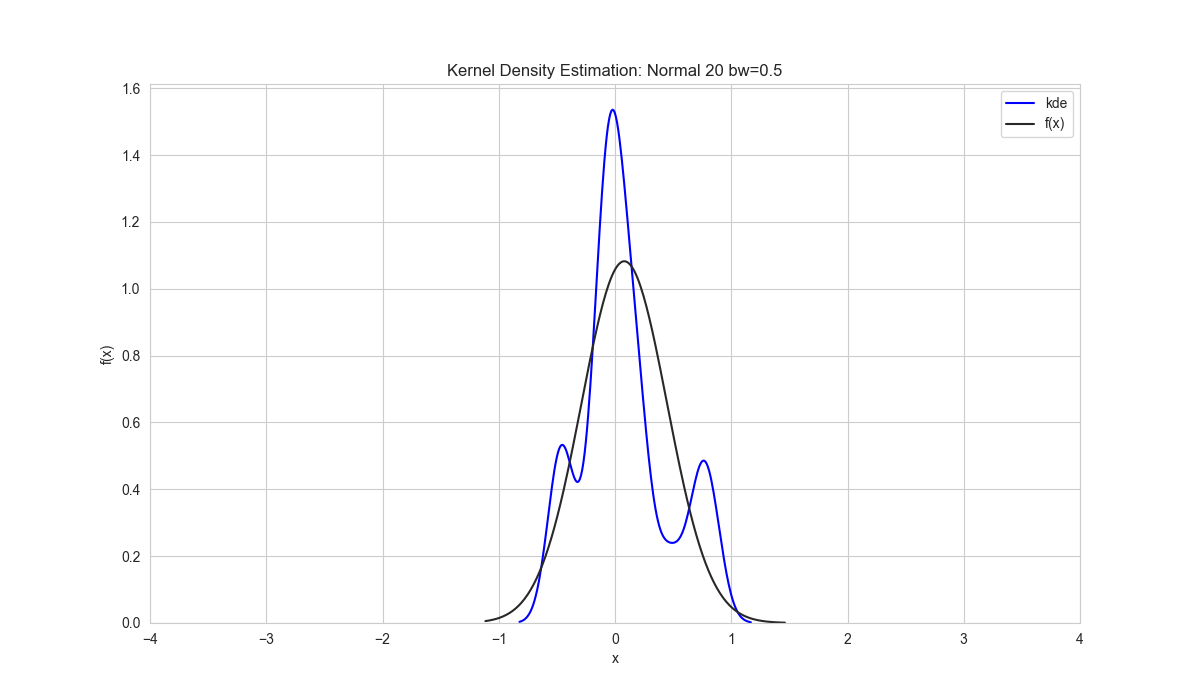
\includegraphics[width=0.3\linewidth]{denNormal200.5}  
\label{fig:norm20_0.5} }  
\subfigure[]{
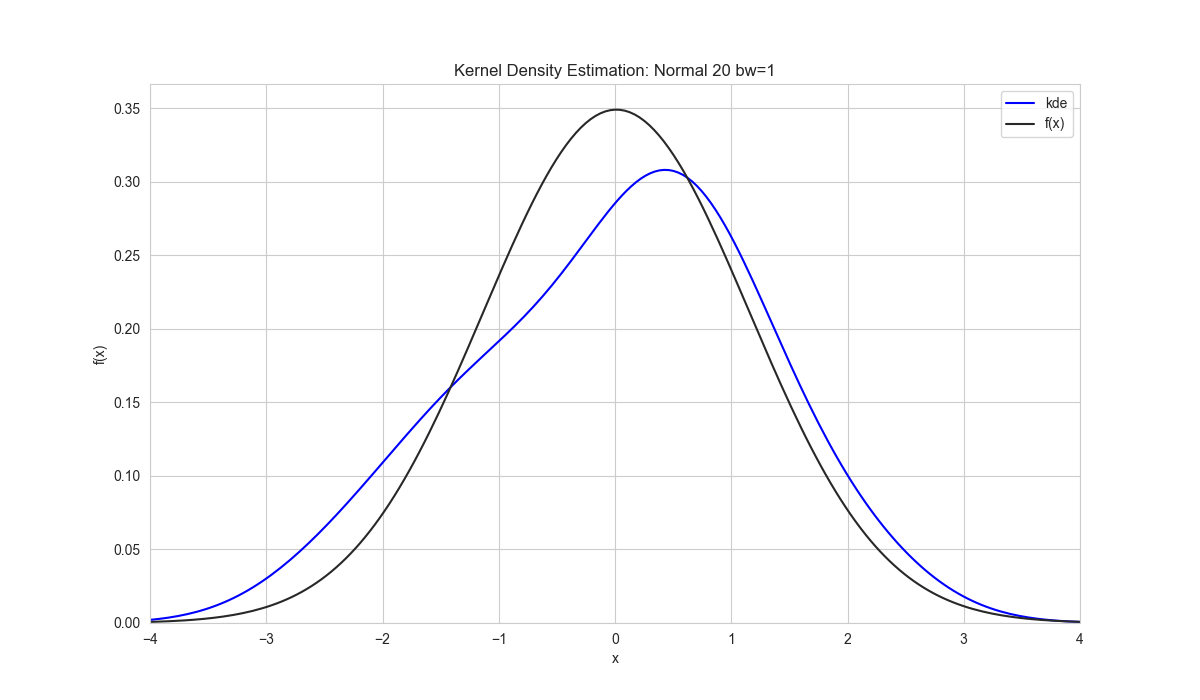
\includegraphics[width=0.3\linewidth]{denNormal201}
\label{fig:norm20_1}  }
\subfigure[]{ 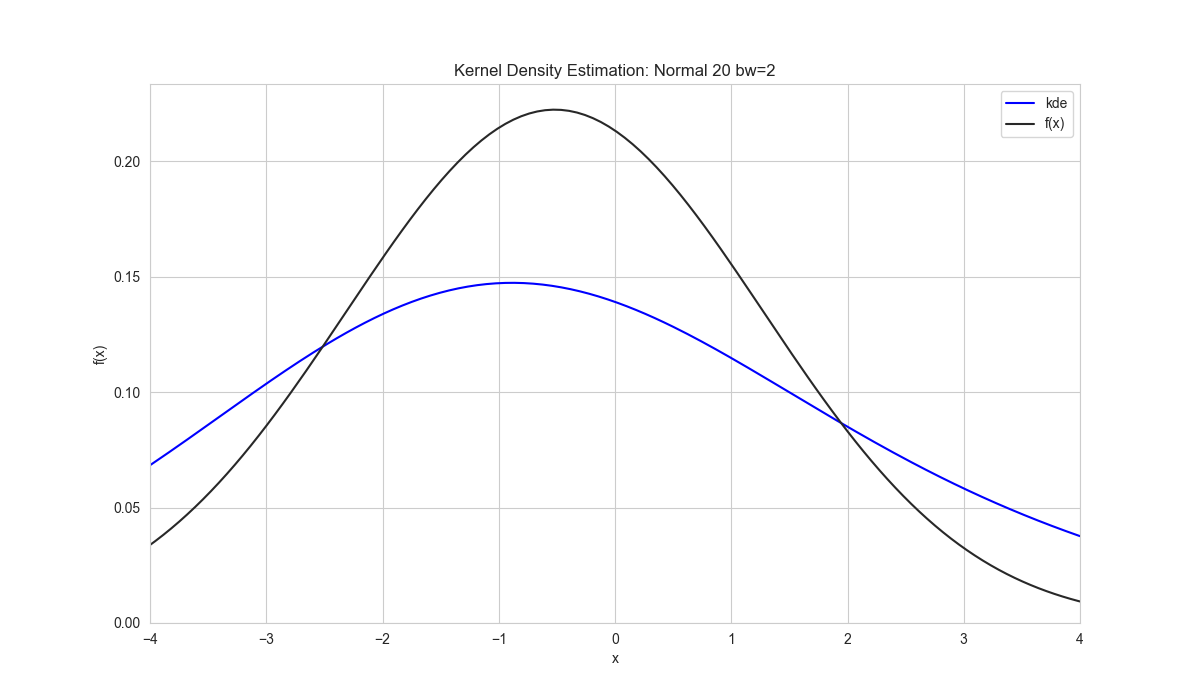
\includegraphics[width=0.3\linewidth]{denNormal202} 
\label{fig:norm20_2} }  
\caption{Ядерная оценка нормального распределения для $n=20$.  
\subref{fig:norm20_0.5} 
при $h=h_n/2$; 
\subref{fig:norm20_1} 
при $h=h_n$; 
\subref{fig:norm20_2}
при $h=2h_n$}
\end{figure}

\begin{figure}[ht!]  
\centering 
\subfigure[]{
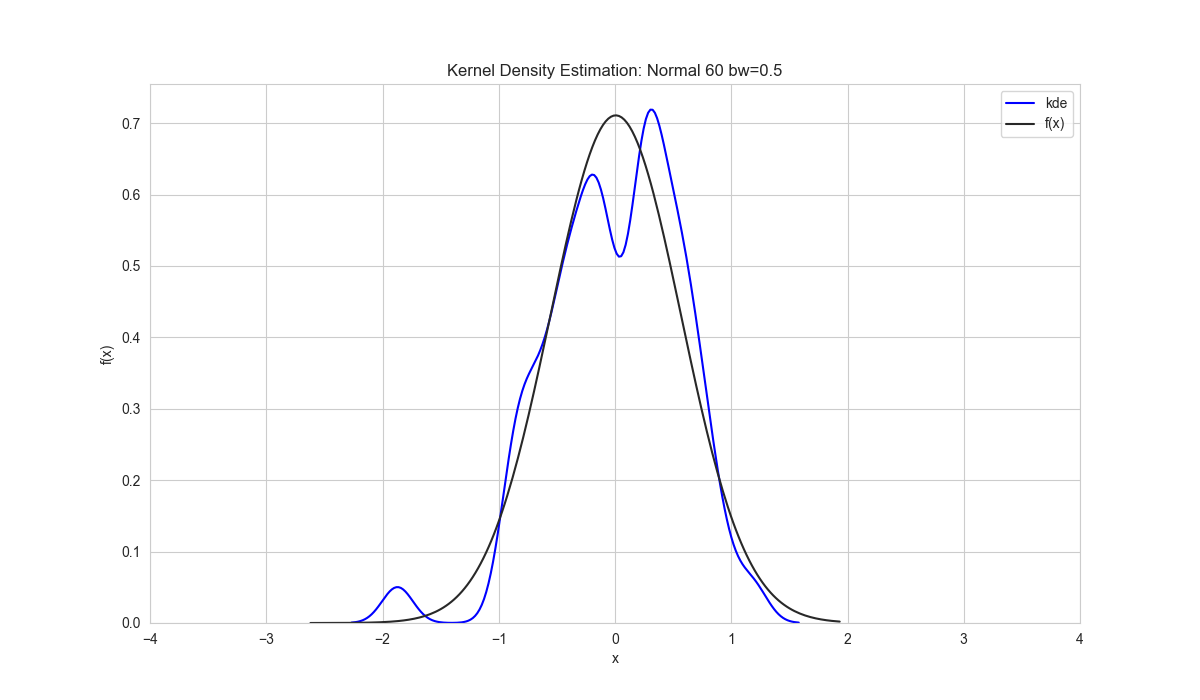
\includegraphics[width=0.3\linewidth]{denNormal600.5}  
\label{fig:norm60_0.5} }  
\subfigure[]{
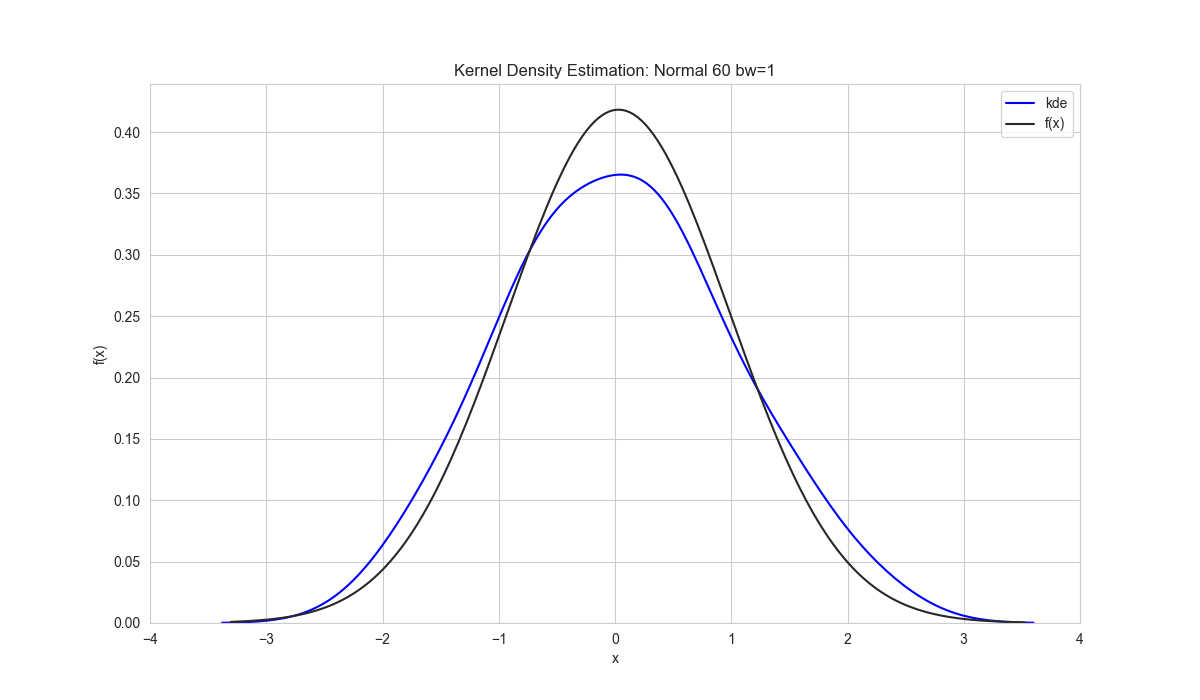
\includegraphics[width=0.3\linewidth]{denNormal601}
\label{fig:norm60_1}  }
\subfigure[]{ 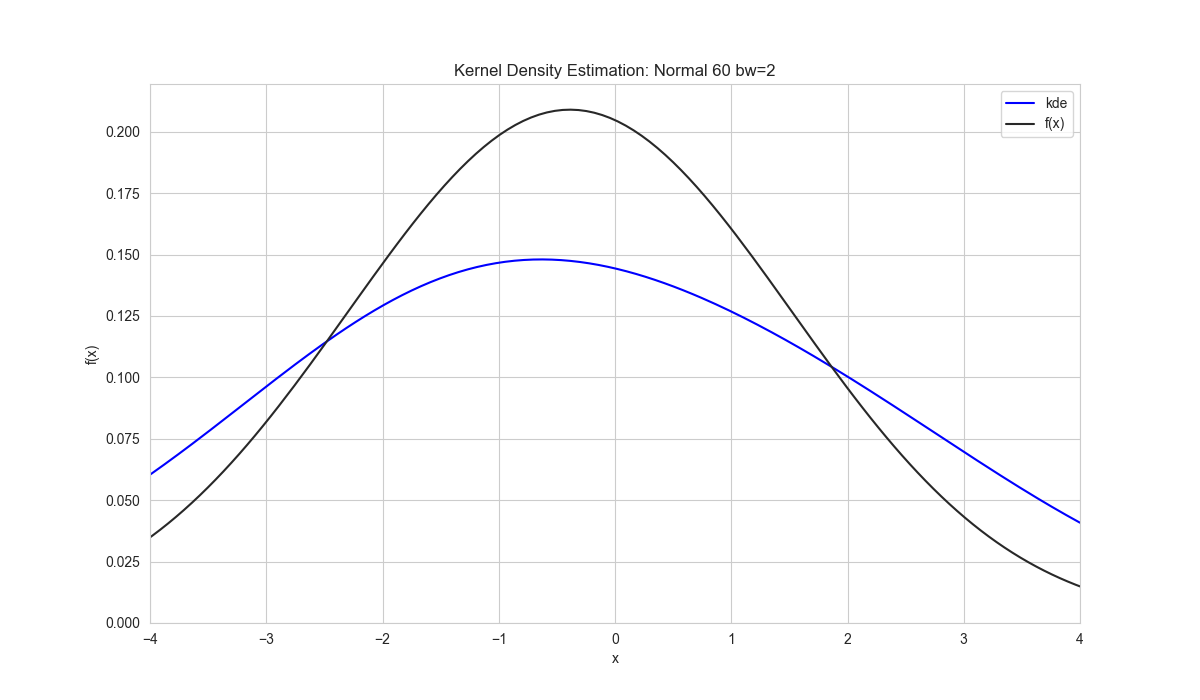
\includegraphics[width=0.3\linewidth]{denNormal602} 
\label{fig:norm60_2} }  
\caption{Ядерная оценка нормального распределения для $n=60$.  
\subref{fig:norm60_0.5} 
при $h=h_n/2$; 
\subref{fig:norm60_1} 
при $h=h_n$; 
\subref{fig:norm60_2}
при $h=2h_n$}
\end{figure}

\begin{figure}[ht!]  
\centering 
\subfigure[]{
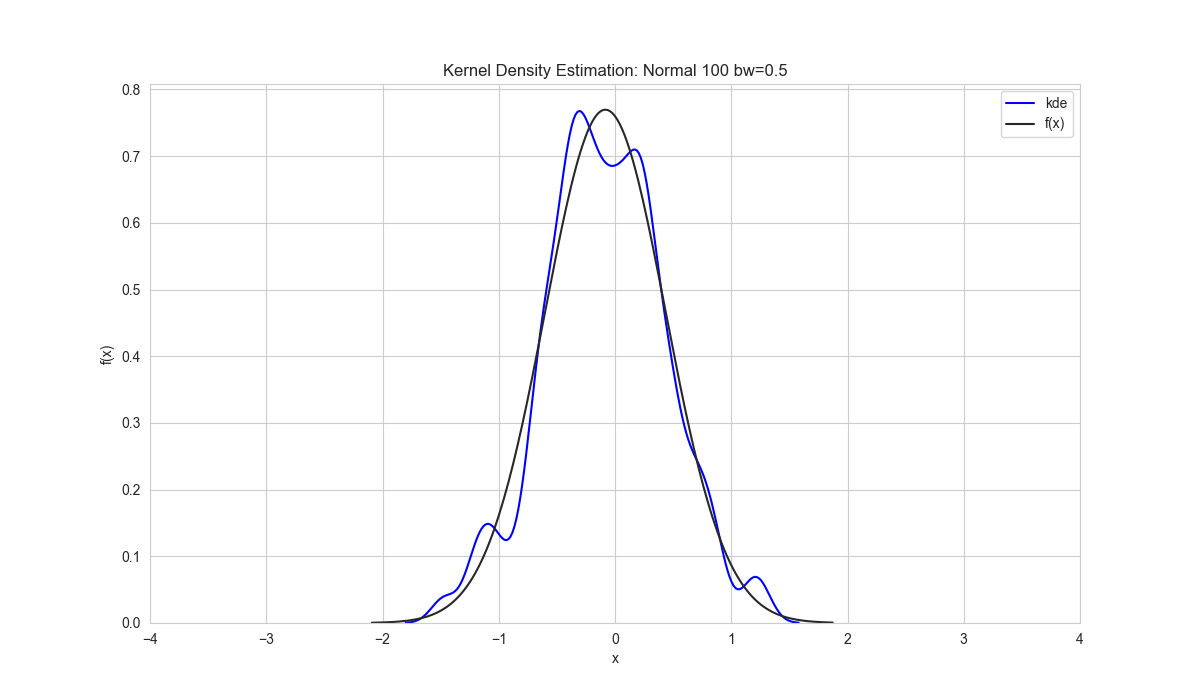
\includegraphics[width=0.3\linewidth]{denNormal1000.5}  
\label{fig:norm100_0.5} }  
\subfigure[]{
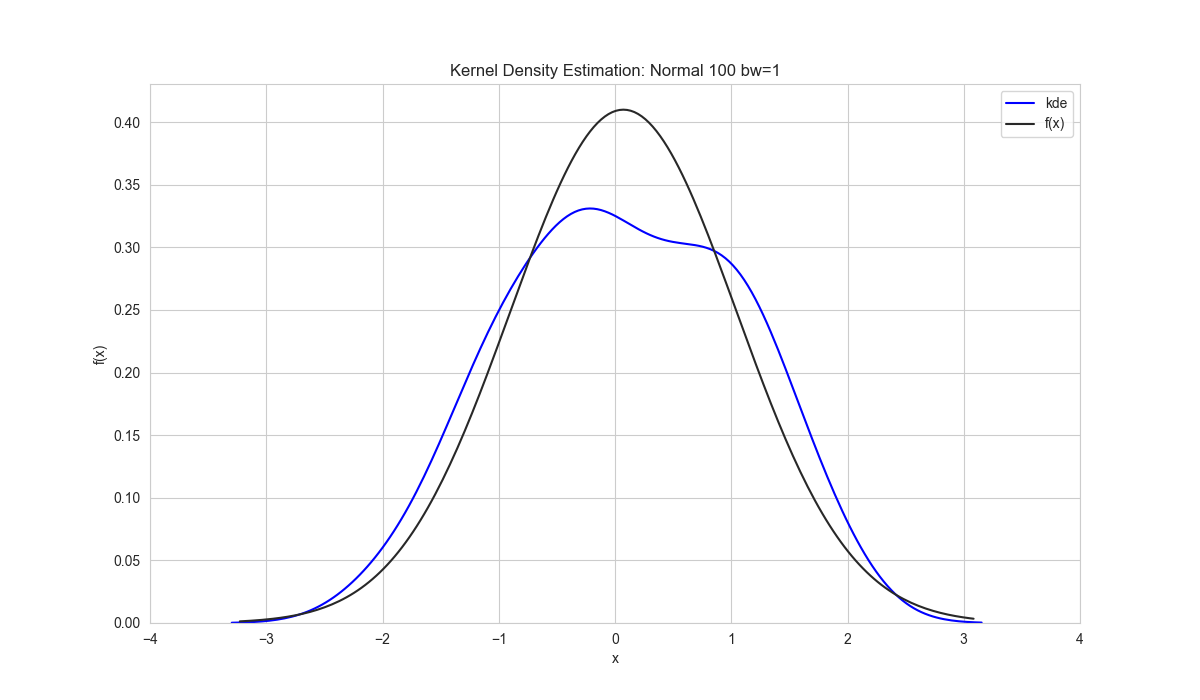
\includegraphics[width=0.3\linewidth]{denNormal1001}
\label{fig:norm100_1}  }
\subfigure[]{ 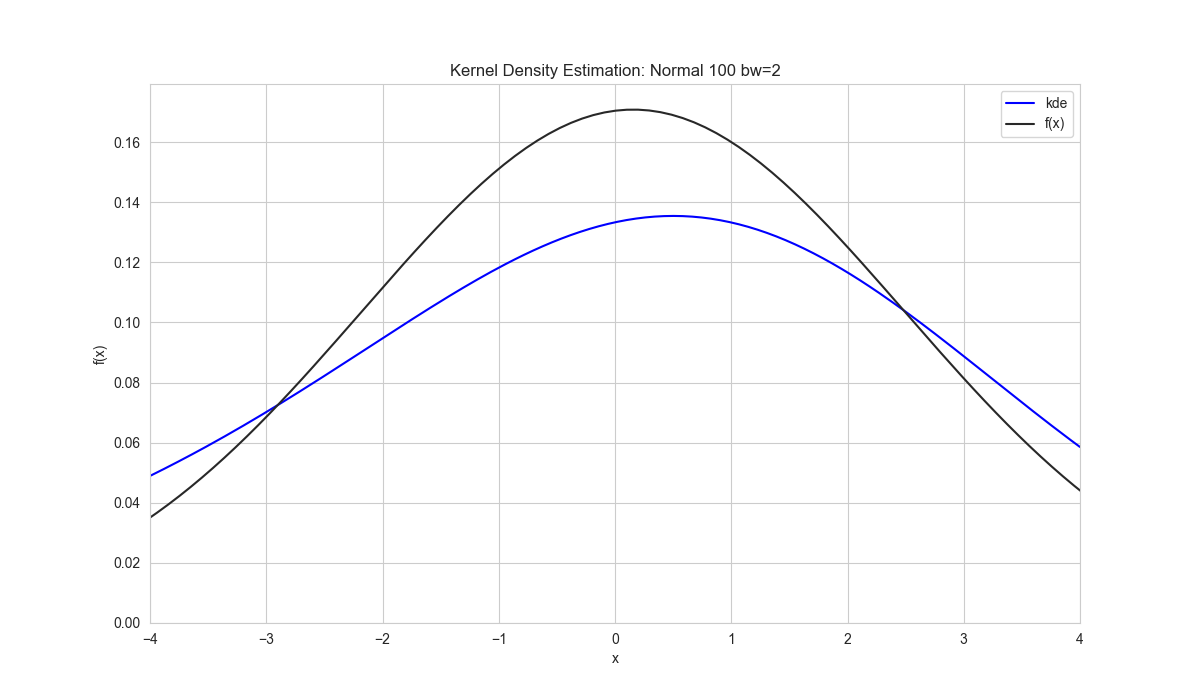
\includegraphics[width=0.3\linewidth]{denNormal1002} 
\label{fig:norm100_2} }  
\caption{Ядерная оценка нормального распределения для $n=100$.  
\subref{fig:norm100_0.5} 
при $h=h_n/2$; 
\subref{fig:norm100_1} 
при $h=h_n$; 
\subref{fig:norm100_2}
при $h=2h_n$}
\end{figure}

\newpage
\subsubsection{Распределение Коши}

\begin{figure}[ht!]  
\centering 
\subfigure[]{
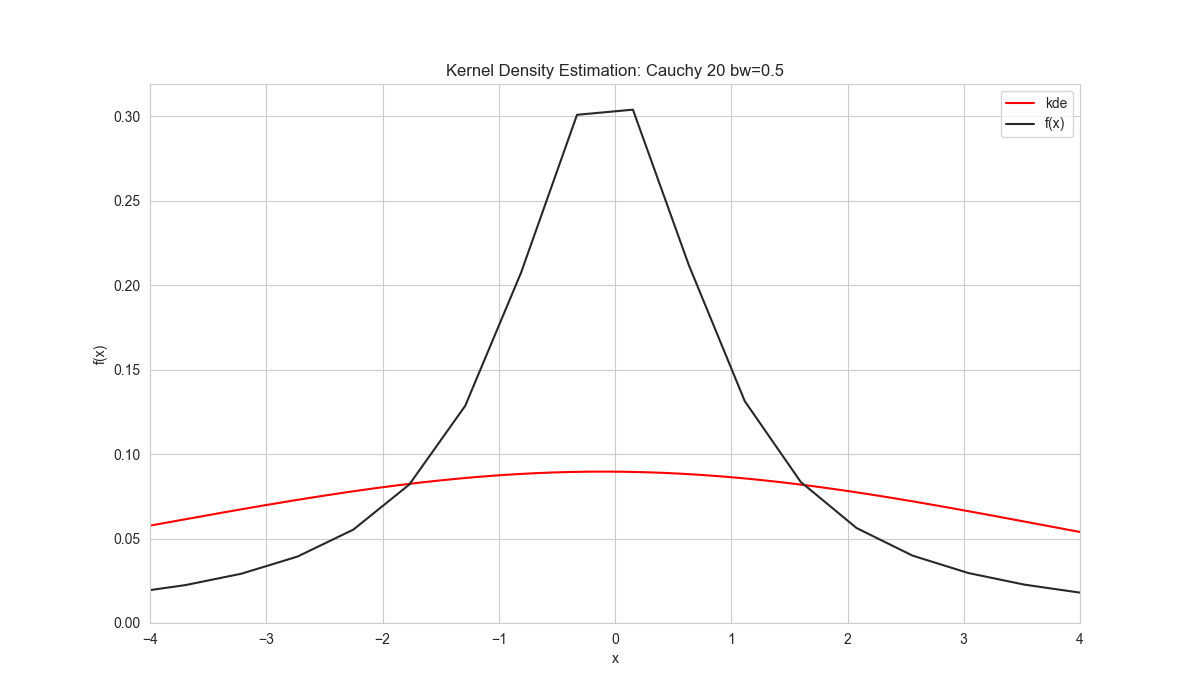
\includegraphics[width=0.3\linewidth]{denCauchy200.5}  
\label{fig:cauchy20_0.5} }  
\subfigure[]{
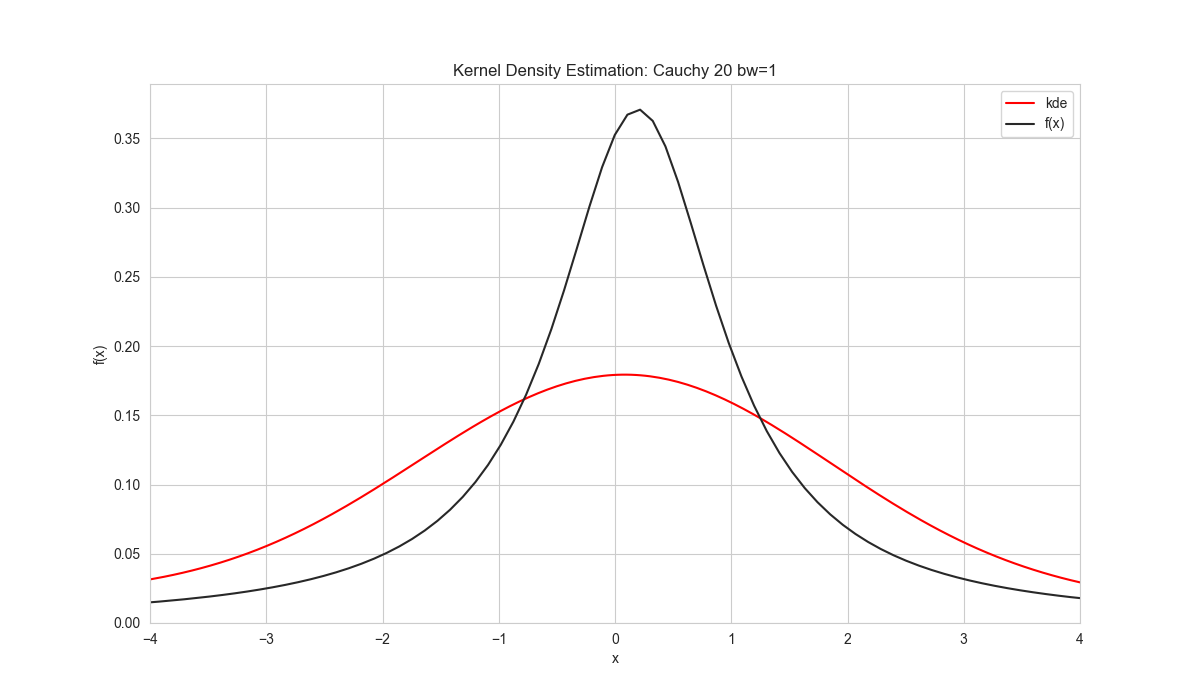
\includegraphics[width=0.3\linewidth]{denCauchy201}
\label{fig:cauchy20_1}  }
\subfigure[]{ 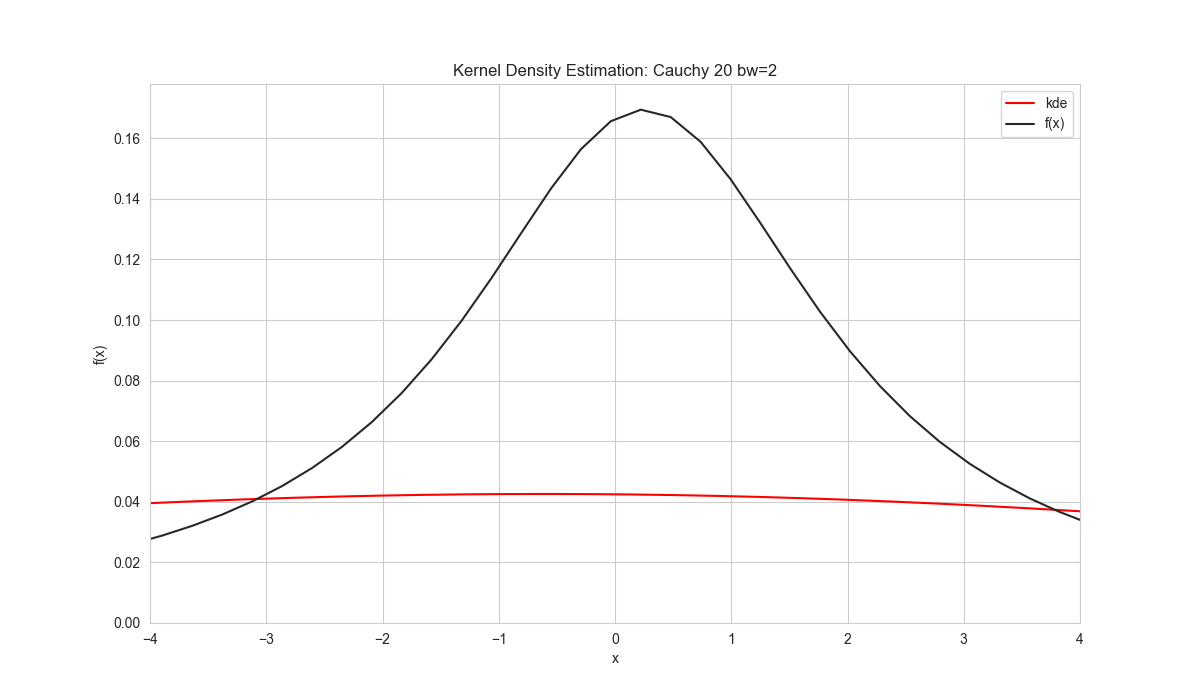
\includegraphics[width=0.3\linewidth]{denCauchy202} 
\label{fig:cauchy20_2} }  
\caption{Ядерная оценка распределения Коши для $n=20$.  
\subref{fig:cauchy20_0.5} 
при $h=h_n/2$; 
\subref{fig:cauchy20_1} 
при $h=h_n$; 
\subref{fig:cauchy20_2}
при $h=2h_n$}
\end{figure}

\begin{figure}[ht!]  
\centering 
\subfigure[]{
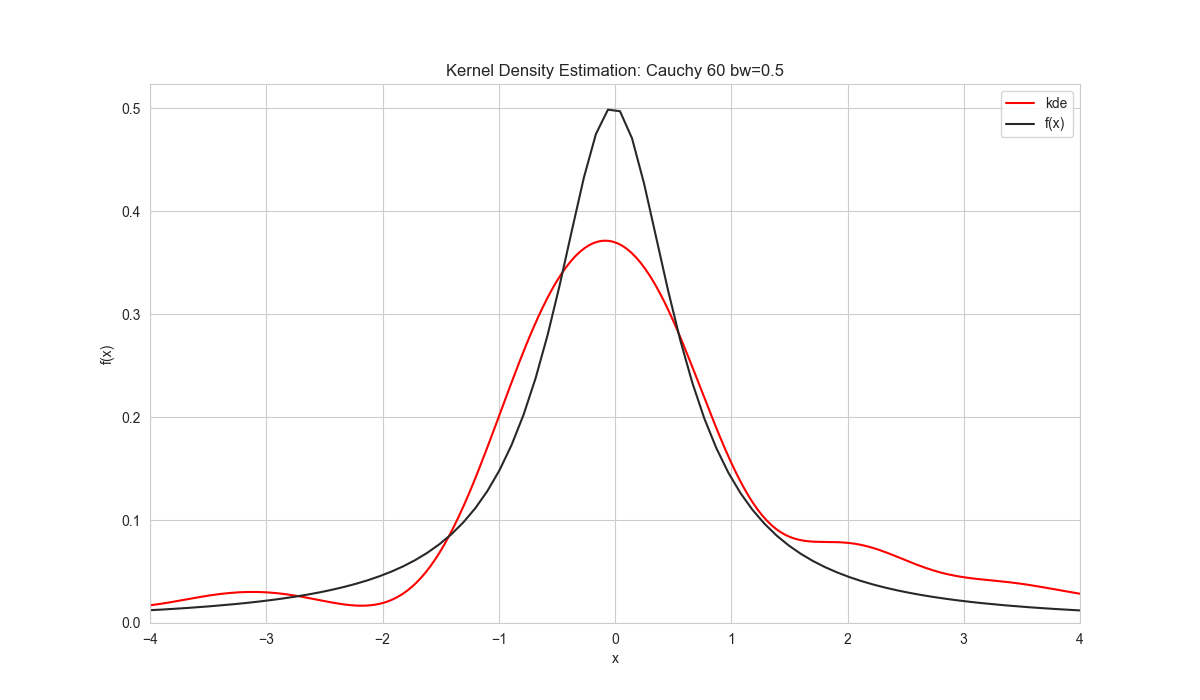
\includegraphics[width=0.3\linewidth]{denCauchy600.5}  
\label{fig:cauchy60_0.5} }  
\subfigure[]{
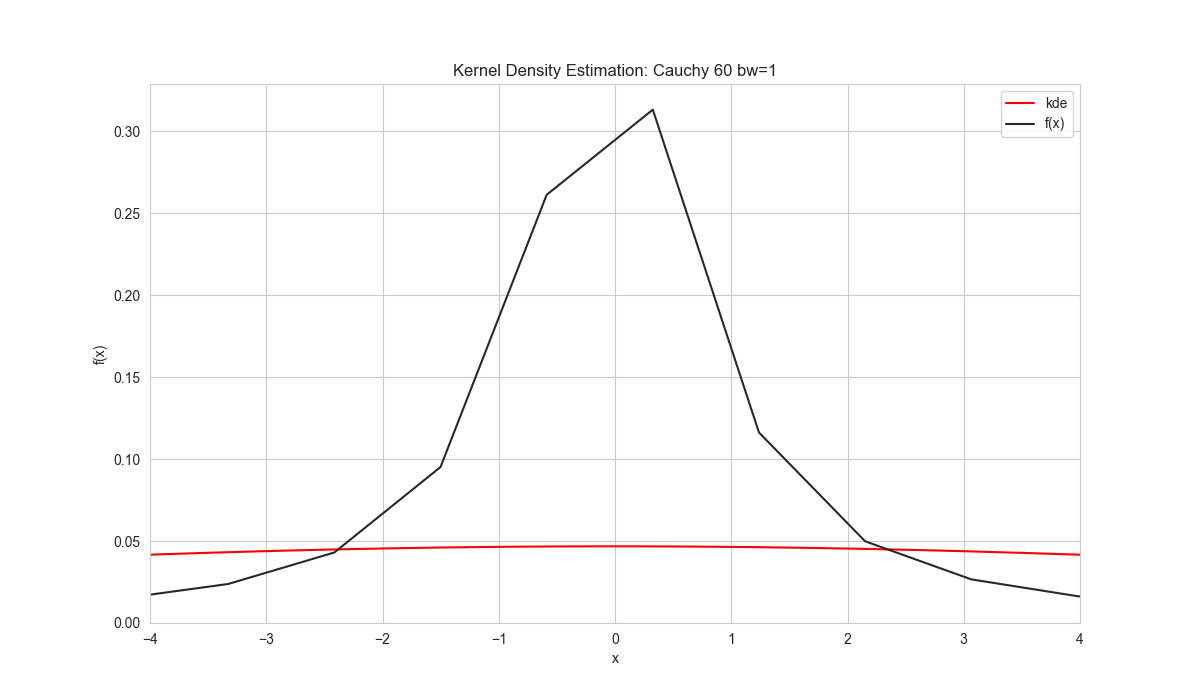
\includegraphics[width=0.3\linewidth]{denCauchy601}
\label{fig:cauchy60_1}  }
\subfigure[]{ 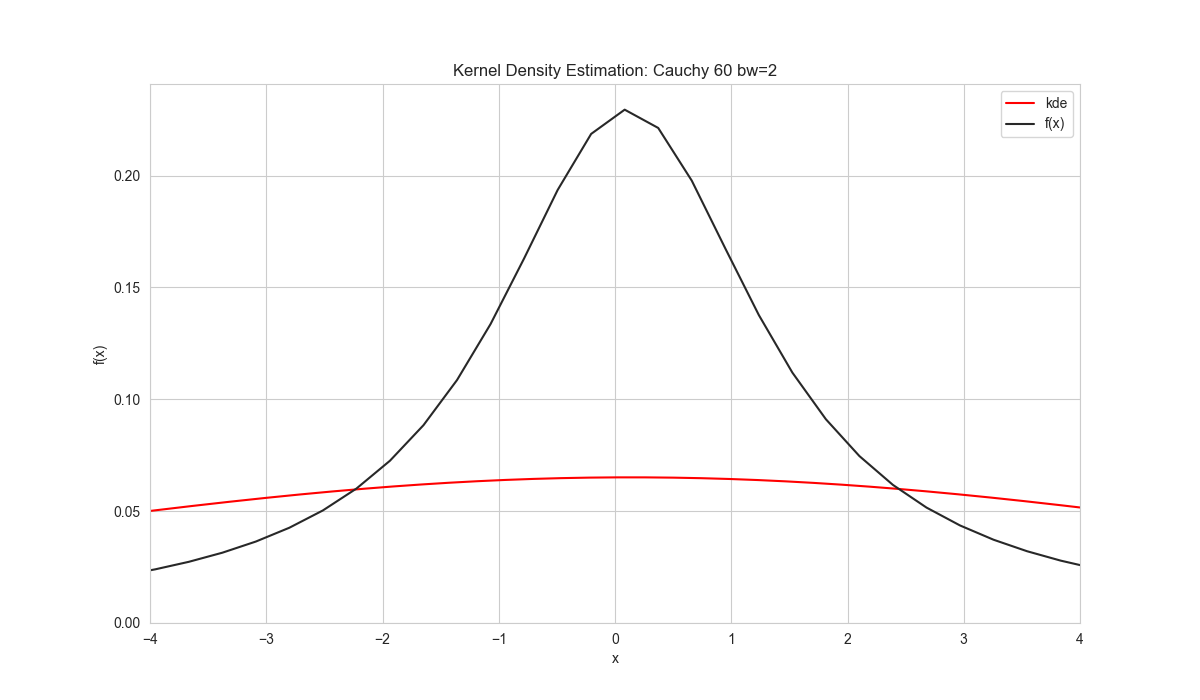
\includegraphics[width=0.3\linewidth]{denCauchy602} 
\label{fig:cauchy60_2} }  
\caption{Ядерная оценка распределения Коши для $n=60$.  
\subref{fig:cauchy60_0.5} 
при $h=h_n/2$; 
\subref{fig:cauchy60_1} 
при $h=h_n$; 
\subref{fig:cauchy60_2}
при $h=2h_n$}
\end{figure}

\begin{figure}[ht!]  
\centering 
\subfigure[]{
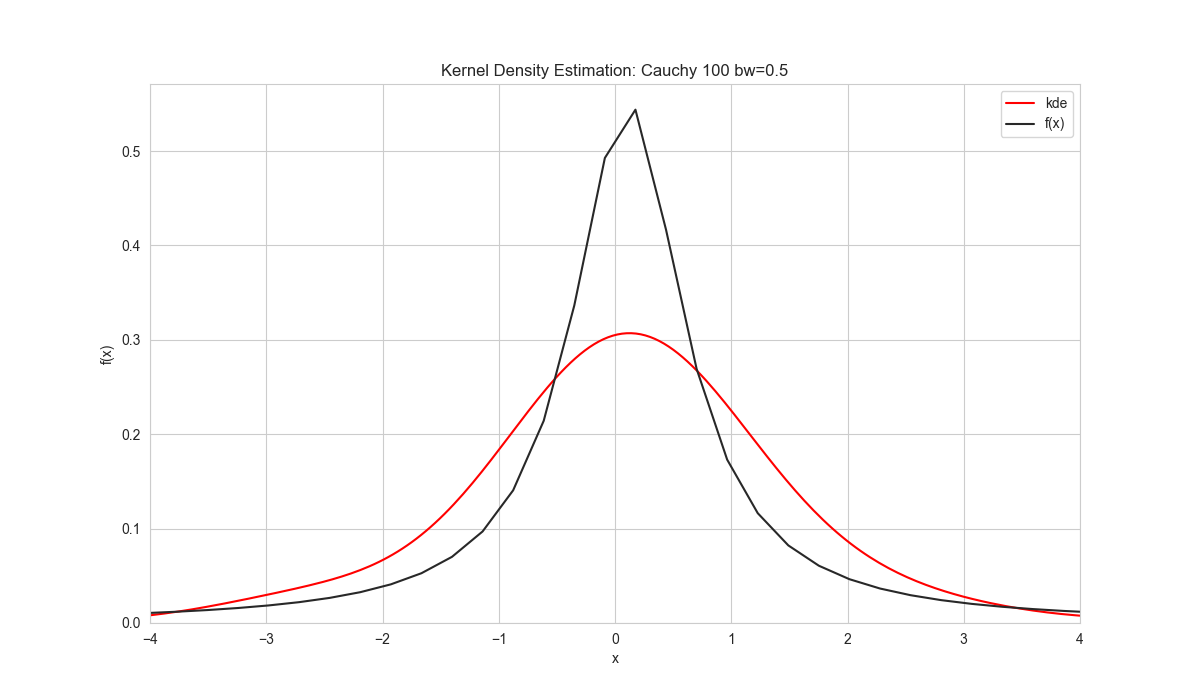
\includegraphics[width=0.3\linewidth]{denCauchy1000.5}  
\label{fig:cauchy100_0.5} }  
\subfigure[]{
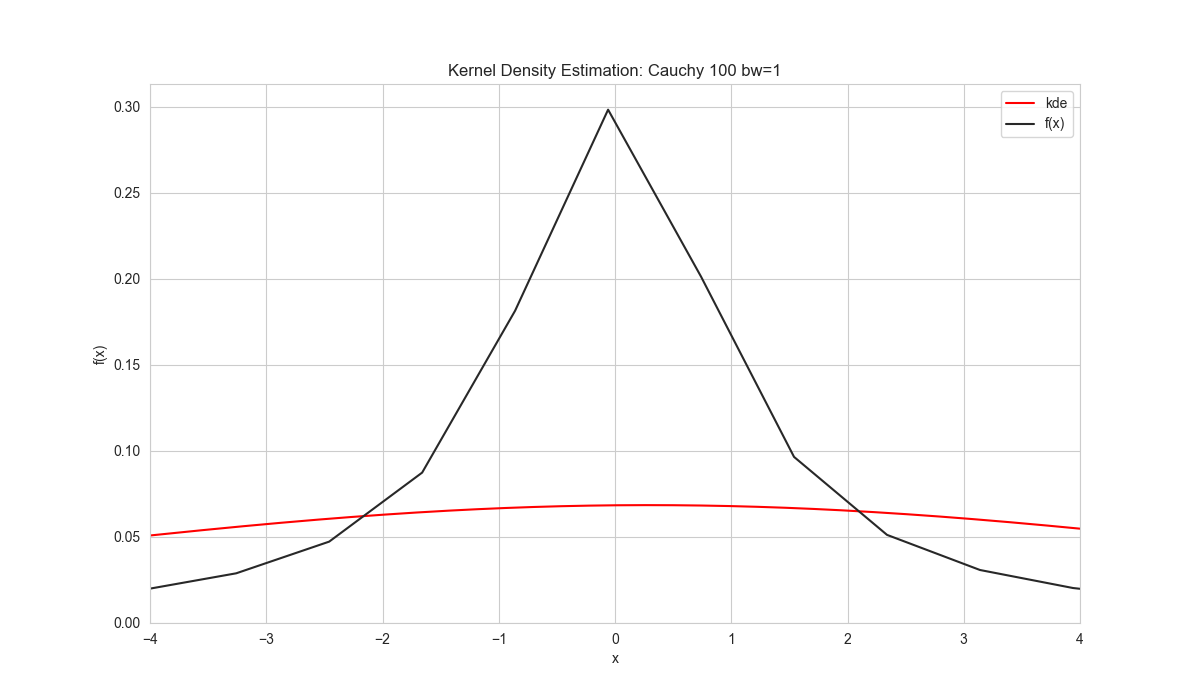
\includegraphics[width=0.3\linewidth]{denCauchy1001}
\label{fig:cauchy100_1}  }
\subfigure[]{ 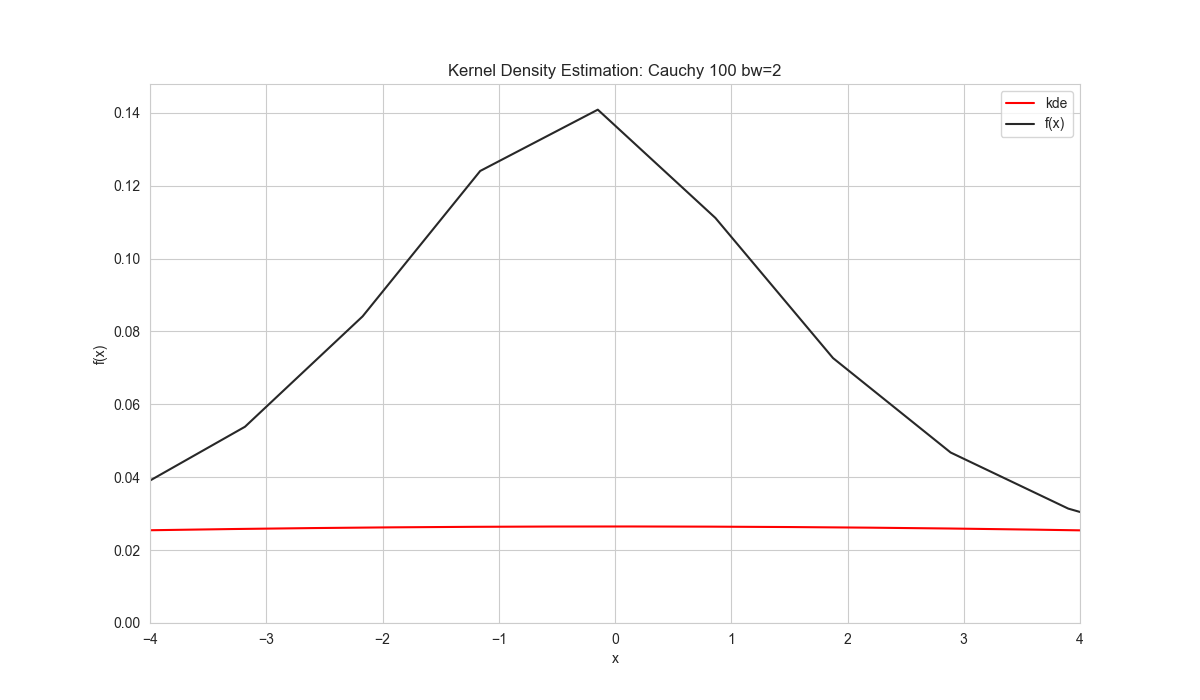
\includegraphics[width=0.3\linewidth]{denCauchy1002} 
\label{fig:cauchy100_2} }  
\caption{Ядерная оценка распределения Коши для $n=100$.  
\subref{fig:cauchy100_0.5} 
при $h=h_n/2$; 
\subref{fig:cauchy100_1} 
при $h=h_n$; 
\subref{fig:cauchy100_2}
при $h=2h_n$}
\end{figure}

\newpage
\subsubsection{Распределение Лапласа}

\begin{figure}[ht!]  
\centering 
\subfigure[]{
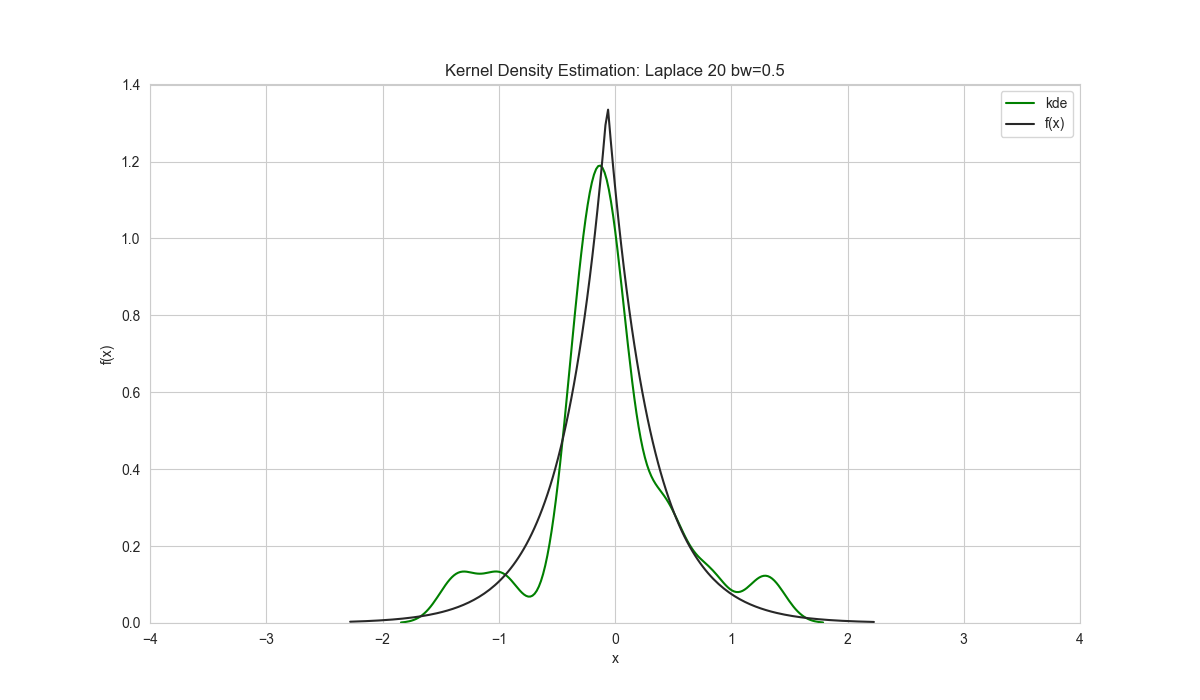
\includegraphics[width=0.3\linewidth]{denLaplace200.5}  
\label{fig:laplace20_0.5} }  
\subfigure[]{
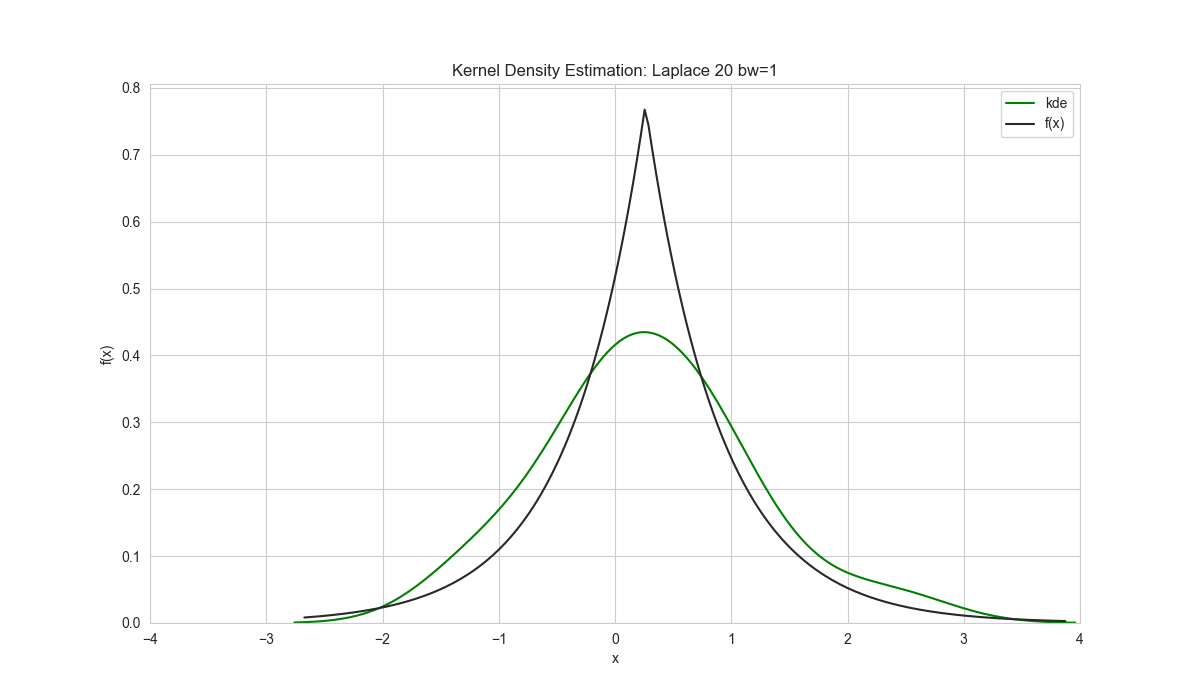
\includegraphics[width=0.3\linewidth]{denLaplace201}
\label{fig:laplace20_1}  }
\subfigure[]{ 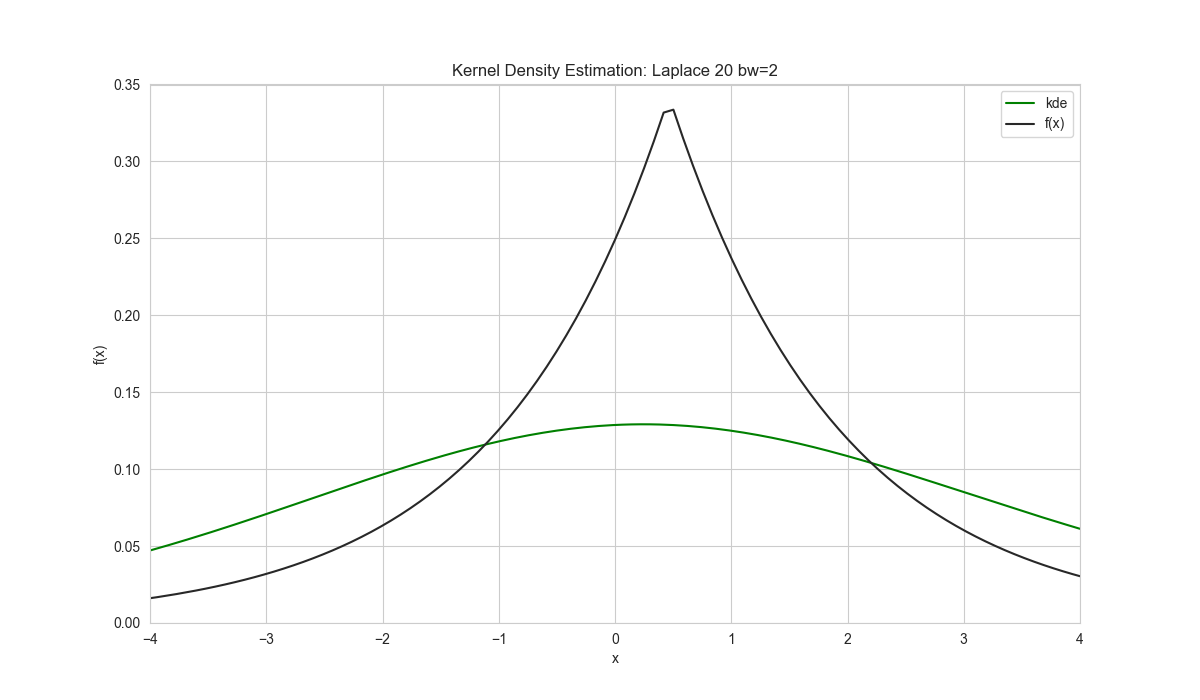
\includegraphics[width=0.3\linewidth]{denLaplace202} 
\label{fig:laplace20_2} }  
\caption{Ядерная оценка распределения Лапласа для $n=20$.  
\subref{fig:laplace20_0.5} 
при $h=h_n/2$; 
\subref{fig:laplace20_1} 
при $h=h_n$; 
\subref{fig:laplace20_2}
при $h=2h_n$}
\end{figure}

\begin{figure}[ht!]  
\centering 
\subfigure[]{
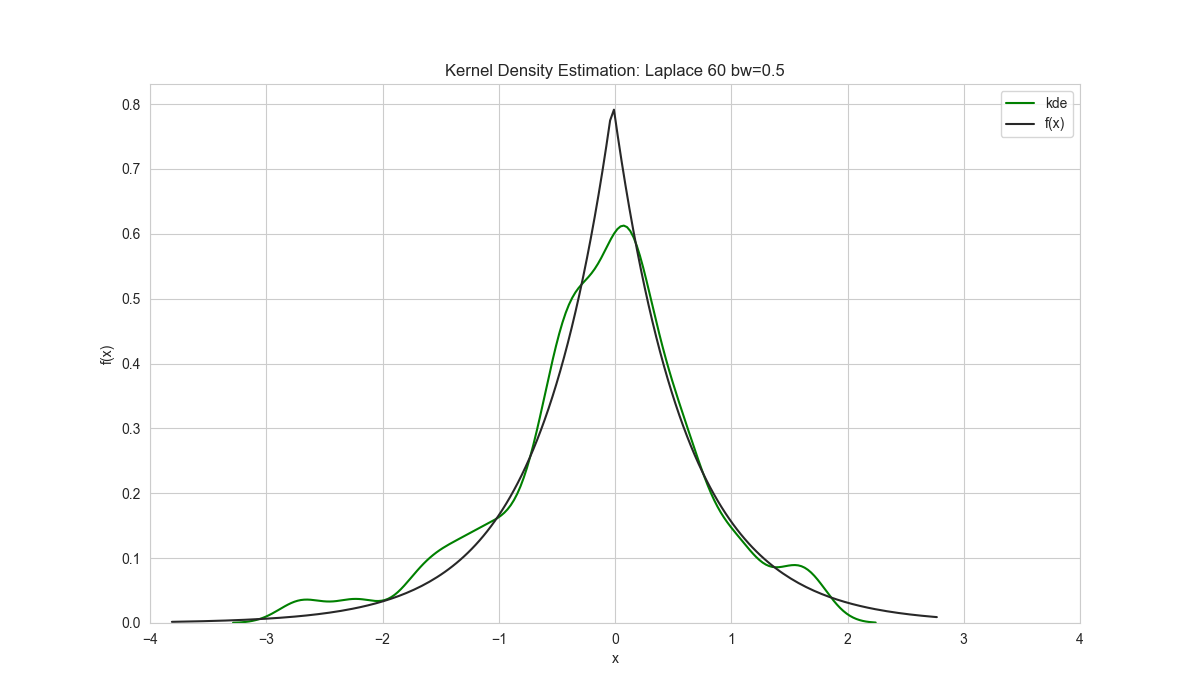
\includegraphics[width=0.3\linewidth]{denLaplace600.5}  
\label{fig:laplace60_0.5} }  
\subfigure[]{
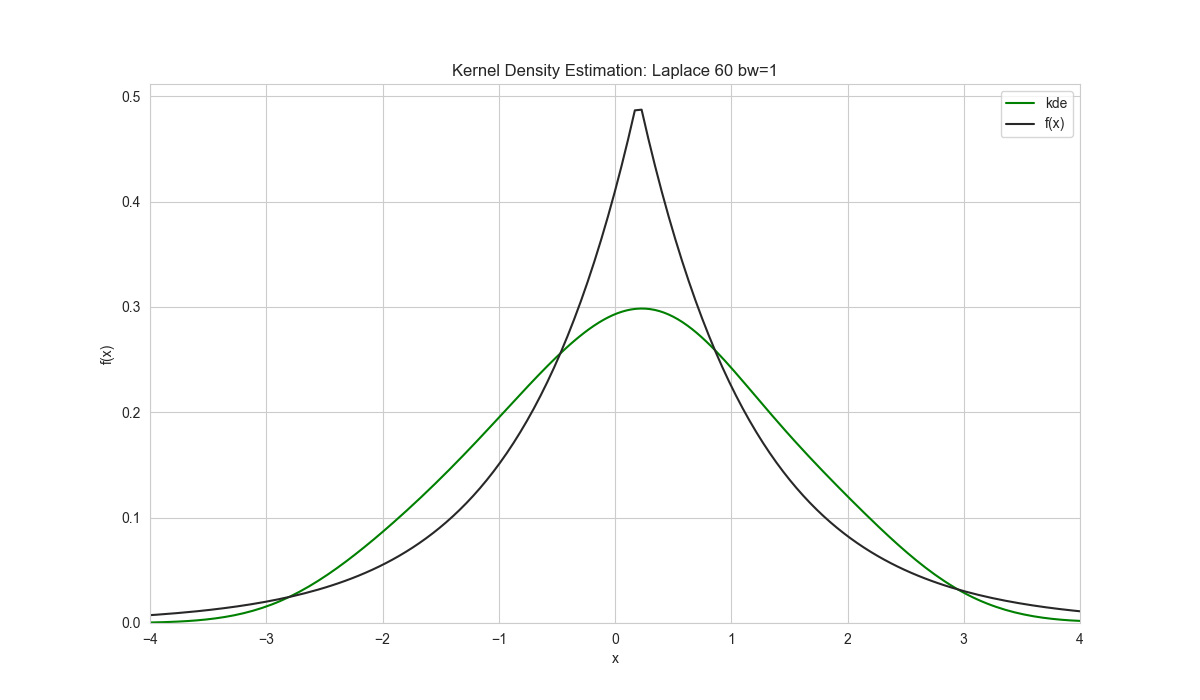
\includegraphics[width=0.3\linewidth]{denLaplace601}
\label{fig:laplace60_1}  }
\subfigure[]{ 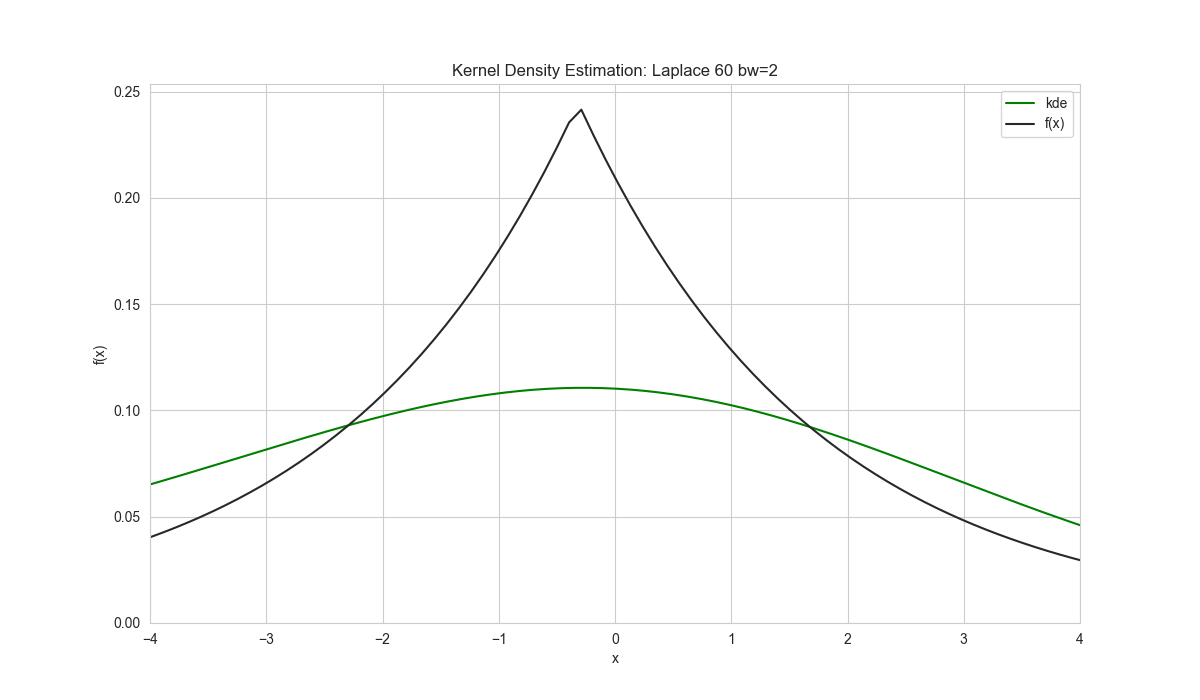
\includegraphics[width=0.3\linewidth]{denLaplace602} 
\label{fig:laplace60_2} }  
\caption{Ядерная оценка распределения Лапласа для $n=60$.  
\subref{fig:laplace60_0.5} 
при $h=h_n/2$; 
\subref{fig:laplace60_1} 
при $h=h_n$; 
\subref{fig:laplace60_2}
при $h=2h_n$}
\end{figure}

\begin{figure}[ht!]  
\centering 
\subfigure[]{
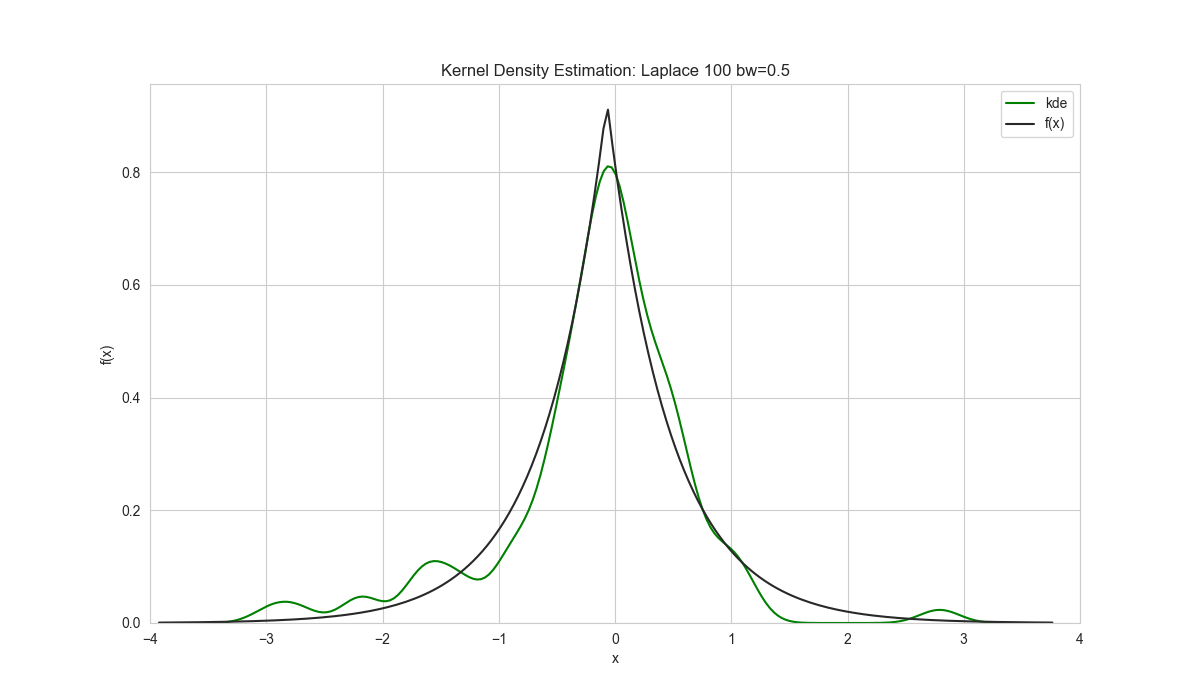
\includegraphics[width=0.3\linewidth]{denLaplace1000.5}  
\label{fig:laplace100_0.5} }  
\subfigure[]{
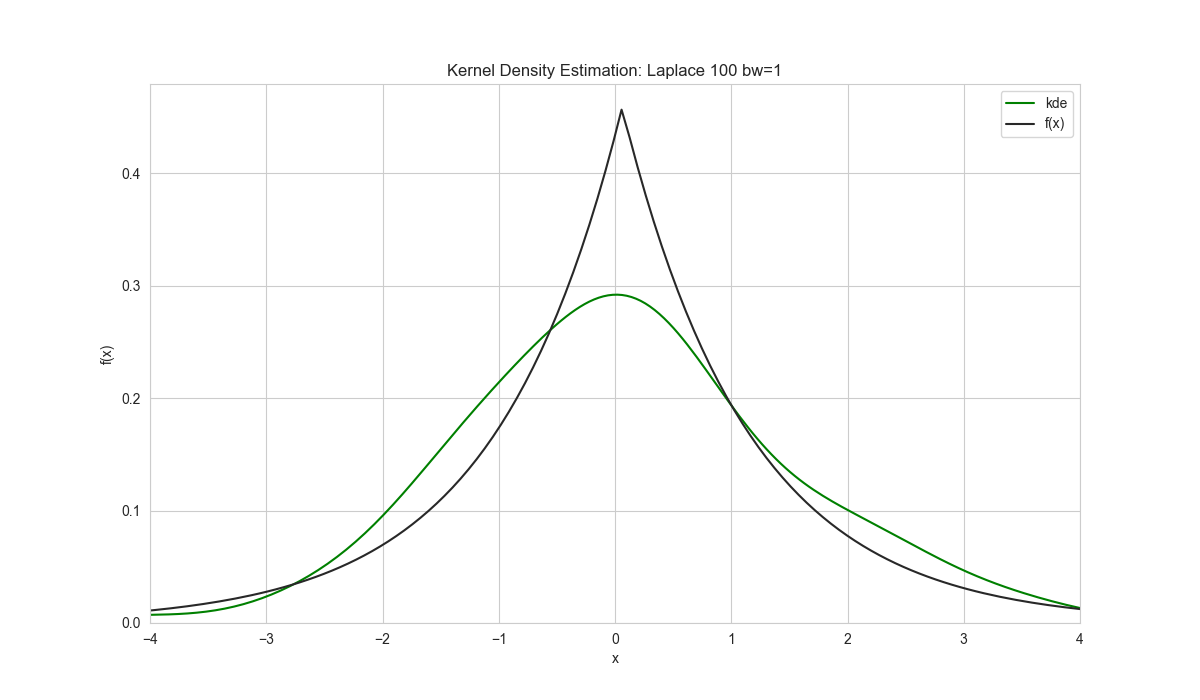
\includegraphics[width=0.3\linewidth]{denLaplace1001}
\label{fig:laplace100_1}  }
\subfigure[]{ 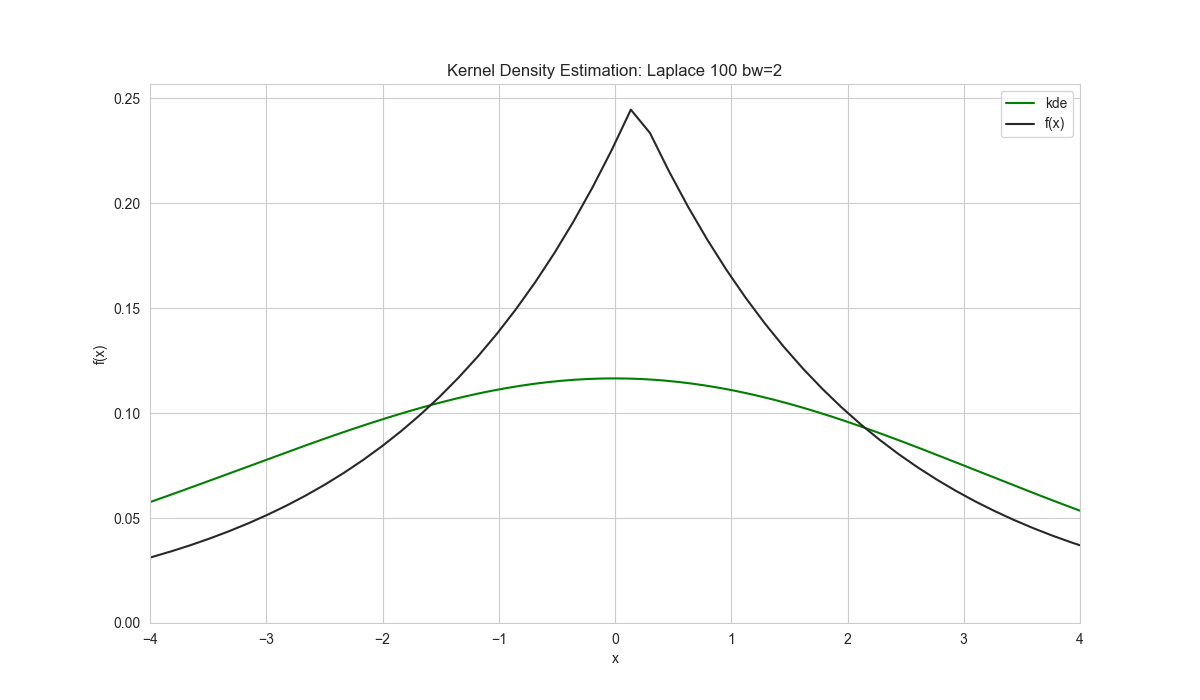
\includegraphics[width=0.3\linewidth]{denLaplace1002} 
\label{fig:laplace100_2} }  
\caption{Ядерная оценка распределения Лапласа для $n=100$.  
\subref{fig:laplace100_0.5} 
при $h=h_n/2$; 
\subref{fig:laplace100_1} 
при $h=h_n$; 
\subref{fig:laplace100_2}
при $h=2h_n$}
\end{figure}

\newpage
\subsubsection{Распределение Пуассона}

\begin{figure}[ht!]  
\centering 
\subfigure[]{
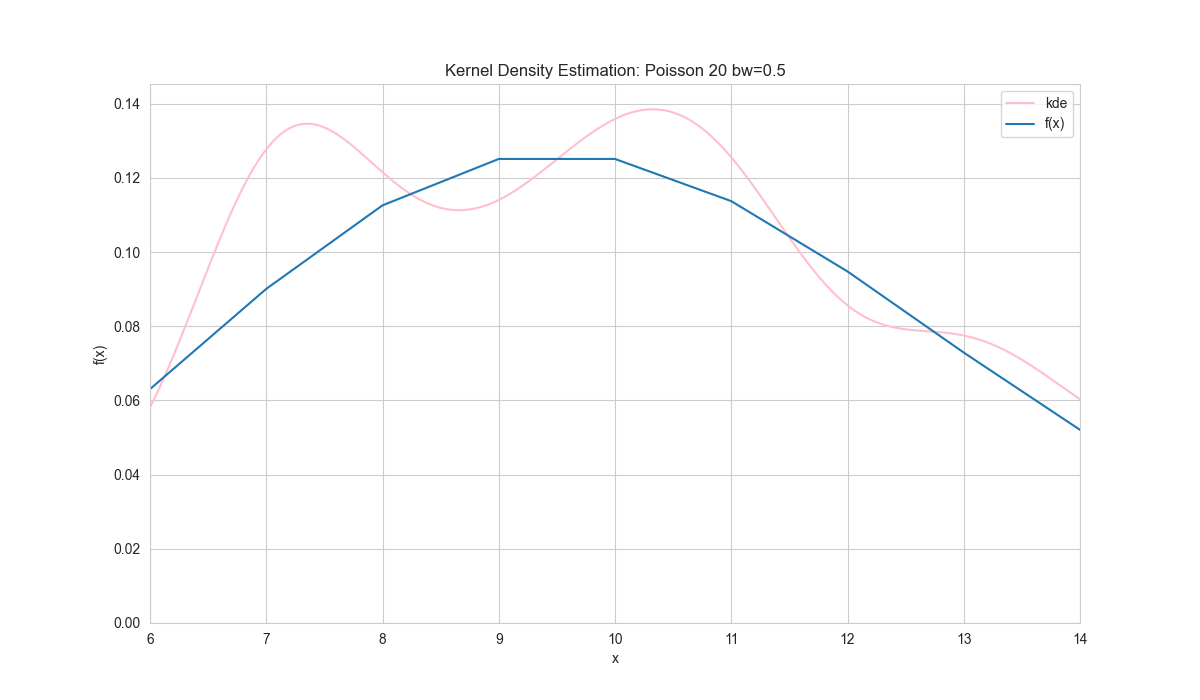
\includegraphics[width=0.3\linewidth]{denPoisson200.5}  
\label{fig:poisson20_0.5} }  
\subfigure[]{
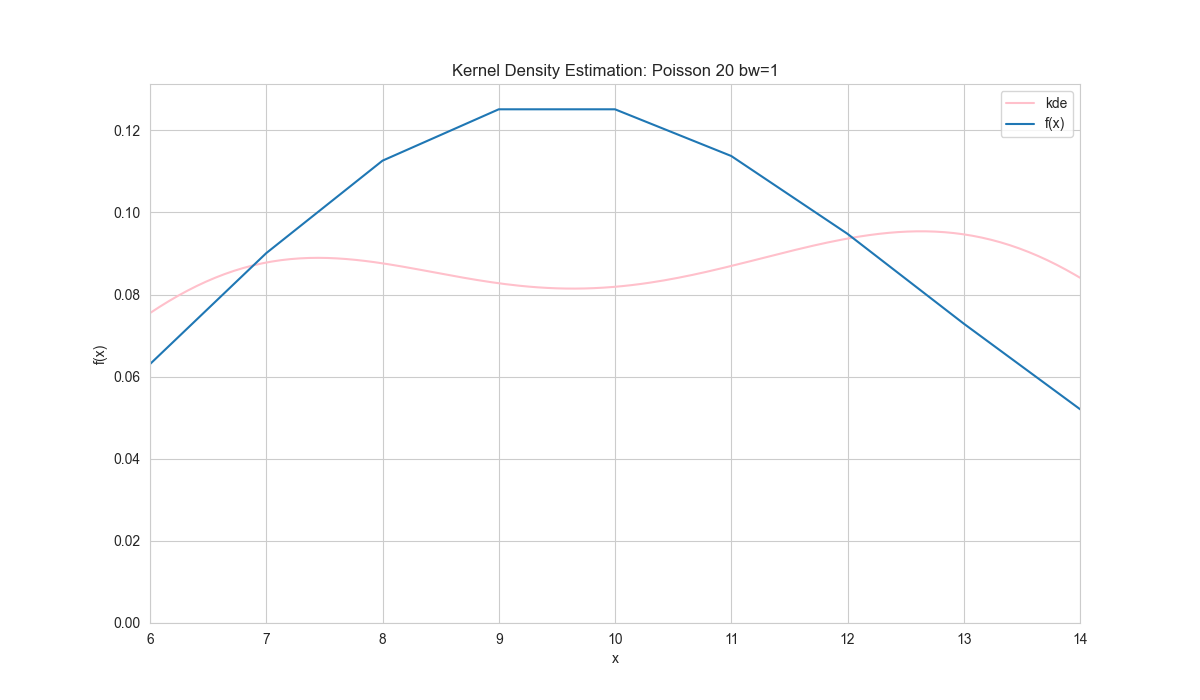
\includegraphics[width=0.3\linewidth]{denPoisson201}
\label{fig:poisson20_1}  }
\subfigure[]{ 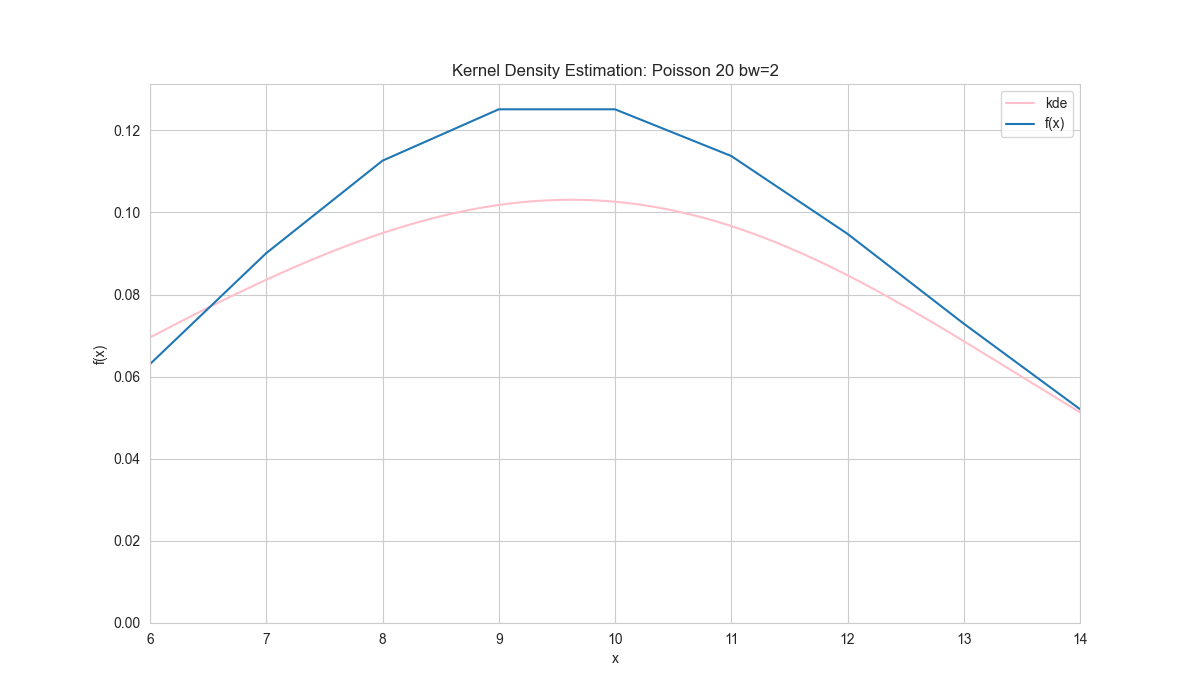
\includegraphics[width=0.3\linewidth]{denPoisson202} 
\label{fig:poisson20_2} }  
\caption{Ядерная оценка распределения Пуассона для $n=20$.  
\subref{fig:poisson20_0.5} 
при $h=h_n/2$; 
\subref{fig:poisson20_1} 
при $h=h_n$; 
\subref{fig:poisson20_2}
при $h=2h_n$}
\end{figure}

\begin{figure}[ht!]  
\centering 
\subfigure[]{
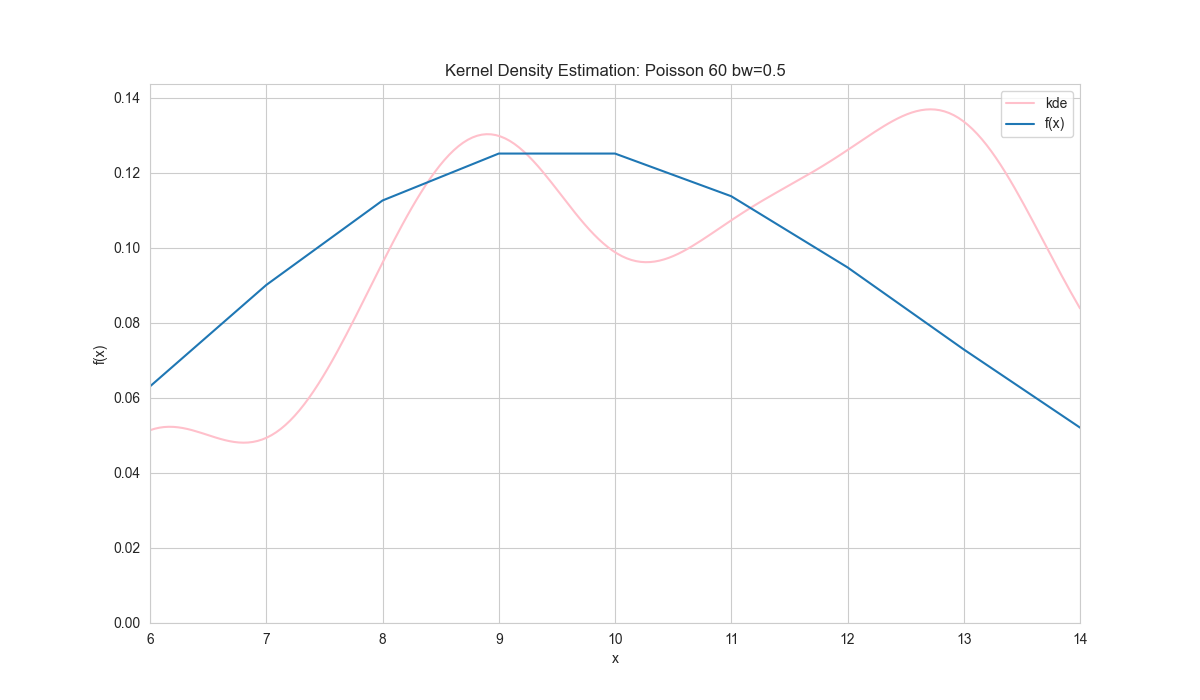
\includegraphics[width=0.3\linewidth]{denPoisson600.5}  
\label{fig:poisson60_0.5} }  
\subfigure[]{
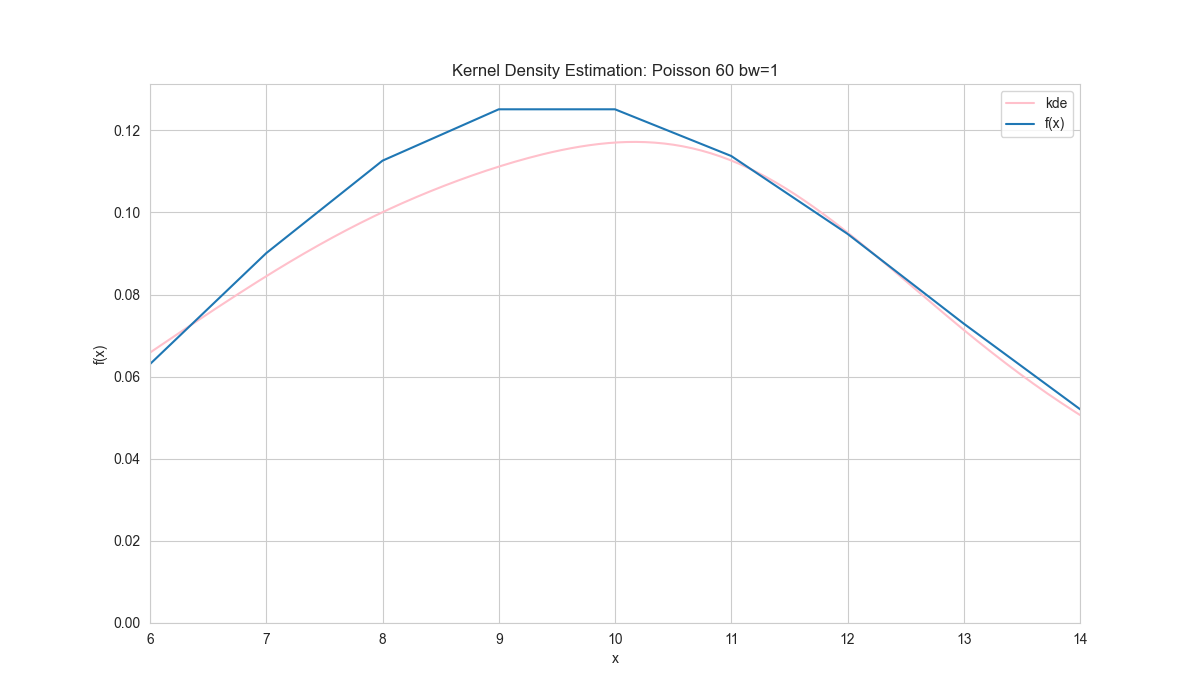
\includegraphics[width=0.3\linewidth]{denPoisson601}
\label{fig:poisson60_1}  }
\subfigure[]{ 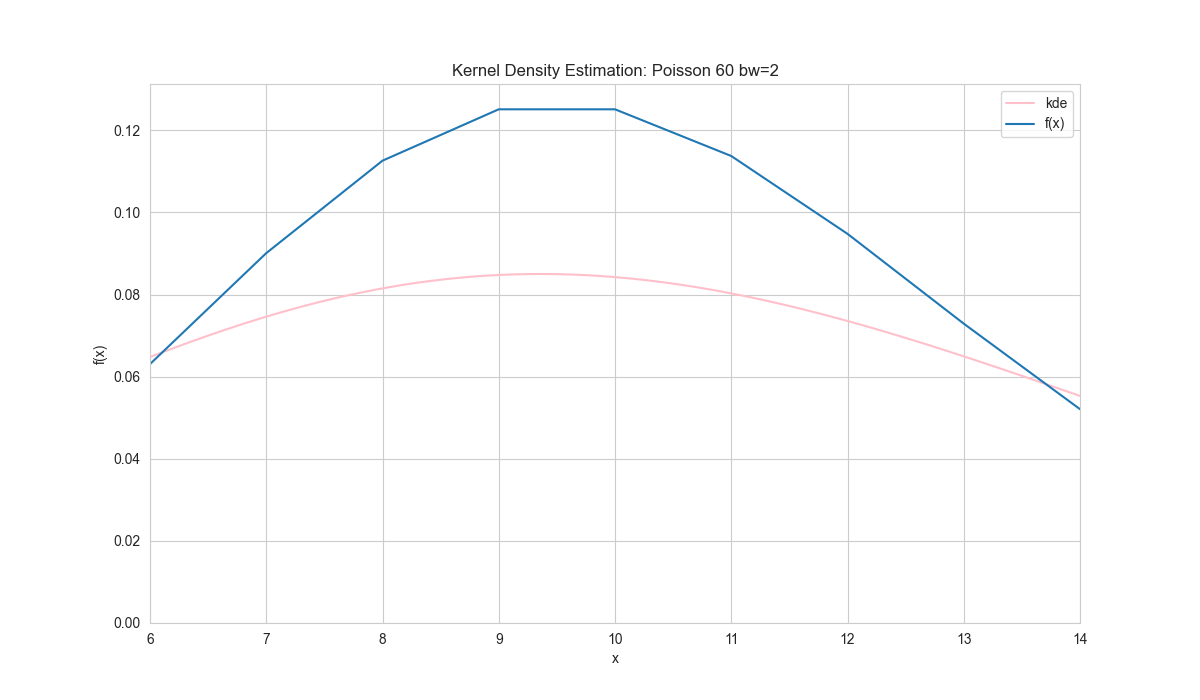
\includegraphics[width=0.3\linewidth]{denPoisson602} 
\label{fig:poisson60_2} }  
\caption{Ядерная оценка распределения Пуассона для $n=60$.  
\subref{fig:poisson60_0.5} 
при $h=h_n/2$; 
\subref{fig:poisson60_1} 
при $h=h_n$; 
\subref{fig:poisson60_2}
при $h=2h_n$}
\end{figure}

\begin{figure}[ht!]  
\centering 
\subfigure[]{
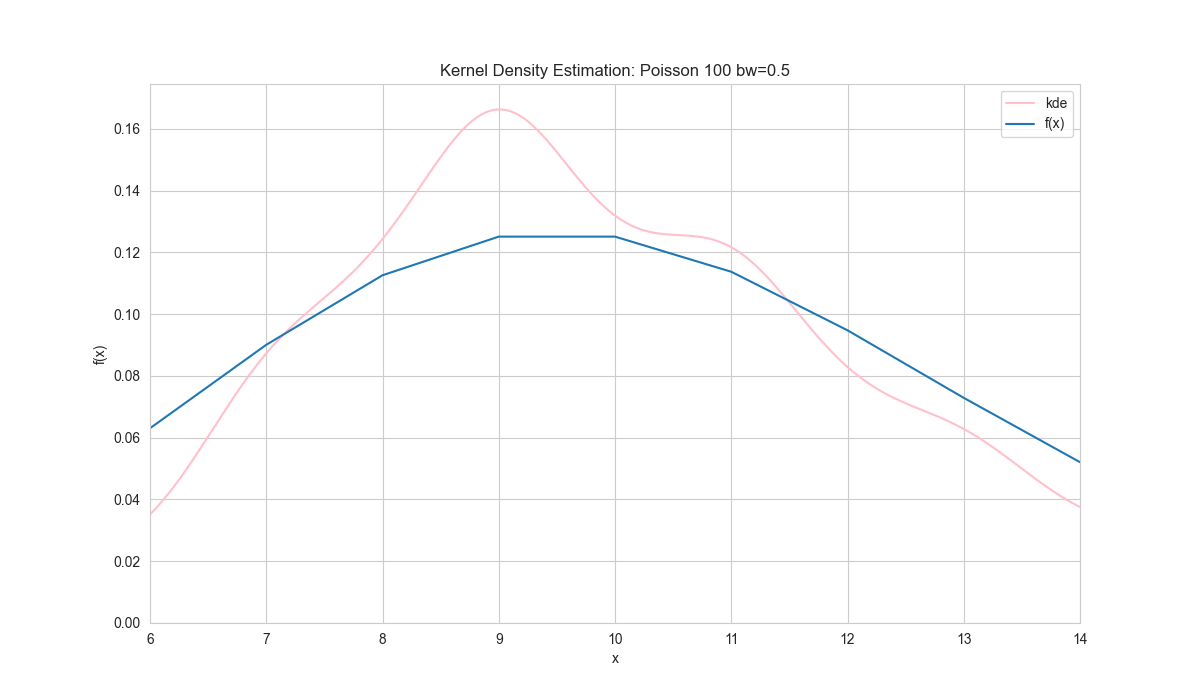
\includegraphics[width=0.3\linewidth]{denPoisson1000.5}  
\label{fig:poisson100_0.5} }  
\subfigure[]{
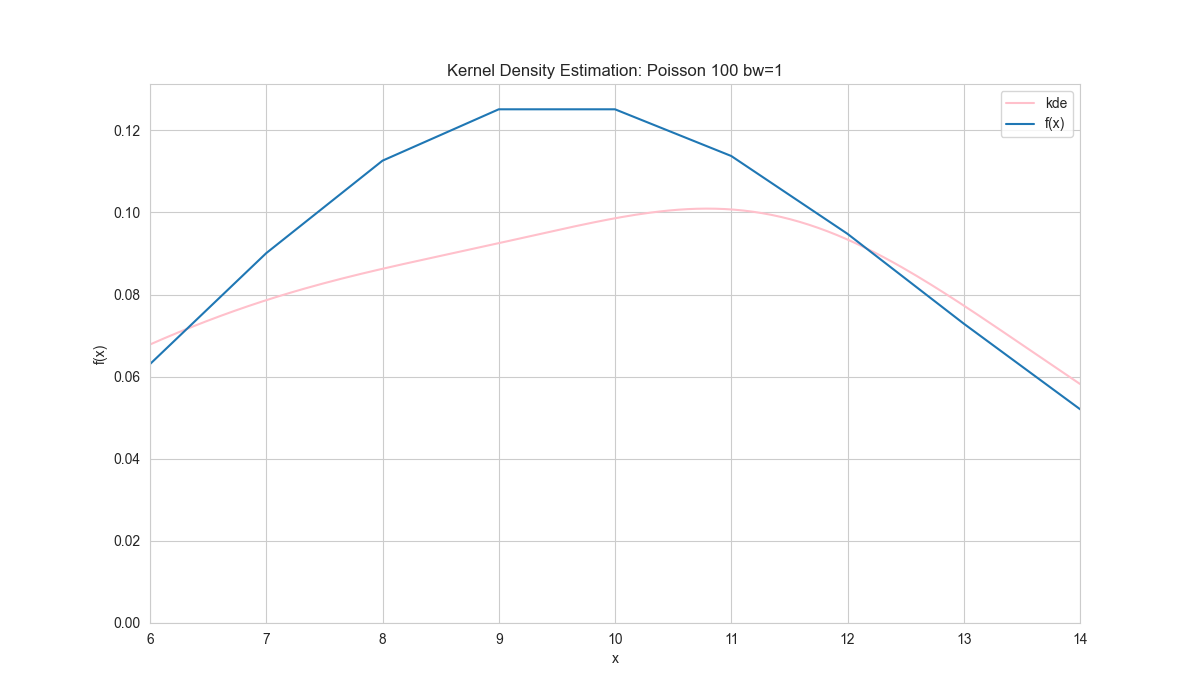
\includegraphics[width=0.3\linewidth]{denPoisson1001}
\label{fig:poisson100_1}  }
\subfigure[]{ \includegraphics[width=0.3\linewidth]{denPoisson1002} 
\label{fig:poisson100_2} }  
\caption{Ядерная оценка распределения Пуассона для $n=100$.  
\subref{fig:poisson100_0.5} 
при $h=h_n/2$; 
\subref{fig:poisson100_1} 
при $h=h_n$; 
\subref{fig:poisson100_2}
при $h=2h_n$}
\end{figure}

\newpage
\subsubsection{Равномерное распределение}

\begin{figure}[ht!]  
\centering 
\subfigure[]{
\includegraphics[width=0.3\linewidth]{denUniform200.5}  
\label{fig:uniform20_0.5} }  
\subfigure[]{
\includegraphics[width=0.3\linewidth]{denUniform201}
\label{fig:uniform20_1}  }
\subfigure[]{ \includegraphics[width=0.3\linewidth]{denUniform202} 
\label{fig:uniform20_2} }  
\caption{Ядерная оценка равномерного распределения для $n=20$.  
\subref{fig:uniform20_0.5} 
при $h=h_n/2$; 
\subref{fig:uniform20_1} 
при $h=h_n$; 
\subref{fig:uniform20_2}
при $h=2h_n$}
\end{figure}

\begin{figure}[ht!]  
\centering 
\subfigure[]{
\includegraphics[width=0.3\linewidth]{denUniform600.5}  
\label{fig:uniform60_0.5} }  
\subfigure[]{
\includegraphics[width=0.3\linewidth]{denUniform601}
\label{fig:uniform60_1}  }
\subfigure[]{ \includegraphics[width=0.3\linewidth]{denUniform602} 
\label{fig:uniform60_2} }  
\caption{Ядерная оценка равномерного распределения для $n=60$.  
\subref{fig:uniform60_0.5} 
при $h=h_n/2$; 
\subref{fig:uniform60_1} 
при $h=h_n$; 
\subref{fig:uniform60_2}
при $h=2h_n$}
\end{figure}

\begin{figure}[ht!]  
\centering 
\subfigure[]{
\includegraphics[width=0.3\linewidth]{denUniform1000.5}  
\label{fig:uniform100_0.5} }  
\subfigure[]{
\includegraphics[width=0.3\linewidth]{denUniform1001}
\label{fig:uniform100_1}  }
\subfigure[]{ \includegraphics[width=0.3\linewidth]{denUniform1002} 
\label{fig:uniform100_2} }  
\caption{Ядерная оценка равномерного распределения для $n=100$.  
\subref{fig:uniform100_0.5} 
при $h=h_n/2$; 
\subref{fig:uniform100_1} 
при $h=h_n$; 
\subref{fig:uniform100_2}
при $h=2h_n$}
\end{figure}

\newpage
\section{Обсуждение}

\subsection{Эмпирическая функция распределения}
Относительно полученных графиков можно сделать вывод, что чем больше мощность выборки тем больше эмпирическая функция распределения приближает функцию распределения выборки. Наибольшее отклонение эмпирической функции от функции распределения можно наблюдать в графиках для распределения Пуассона

\subsection{Ядерная оценка плотности}
Для каждой выборки было построено несколько графиков с разным параметром сглаживания $h$. Из чего можно сделать выбор что для определенных распределений лучше выбирать разные параметры $h$:
\begin{itemize}
	\item Нормальное распределение: $h=h_n$
	\item Распределение Коши: $h=h_n$
	\item Распределение Лапласа: $h=h_n/2$
	\item Распределение Пуассона: $h=2h_n$
	\item Равномерное распределение: $h=2h_n$
\end{itemize}
Данные значения будут сильнее приближать ядерную оценку плотности к плотности выборки

\newpage
\begin{thebibliography}{4}
\addcontentsline{toc}{section}{\bibname}
\bibitem{cauchy}
Документация бибилиотеки scipy.stats.cauchy. 
\\ URL: https://docs.scipy.org/doc/scipy/reference/generated/scipy.stats.cauchy.html
\bibitem{laplace}
Документация бибилиотеки scipy.stats.laplace. 
\\ URL: https://docs.scipy.org/doc/scipy/reference/generated/scipy.stats.laplace.html
\bibitem{poisson}
Документация бибилиотеки scipy.stats.poisson.
\\ URL: https://docs.scipy.org/doc/scipy/reference/generated/scipy.stats.poisson.html
\bibitem{uniform}
Документация бибилиотеки scipy.stats.uniform.
\\ URL: https://docs.scipy.org/doc/scipy/reference/generated/scipy.stats.uniform.html
\end{thebibliography}
\end{document}
